%\documentclass[11pt]{book}
\documentclass[10pt]{article}
%\documentclass[11pt]{amsart}
%\documentclass[preprint,12pt]{elsarticle}

\usepackage{etex}
\usepackage{standalone}
\usepackage{tikz}
% !TEX root=img/arguments_and_attack.tex

% \usetikzlibrary{external} 
% \tikzexternalize[prefix=tikz/] 

\usetikzlibrary{calc}
\usetikzlibrary{arrows}
\usetikzlibrary{arrows.meta}
\usetikzlibrary{decorations.markings}
% \usetikzlibrary{intersections}
\usetikzlibrary{fit}
\usetikzlibrary{shapes}
% \usetikzlibrary{trees}


\tikzset{
	every path/.style={thick},
	align=center,
	observed/.style={
		fill=black!20,
	},
	bn/.style={
		draw,
		ellipse,
		-{Triangle[angle=60:6pt 0]}
	},
	scn/.style={
		draw,
		rectangle,
		% signal,
		% signal from=west,
		% signal pointer angle=120,
		-{Triangle[angle=60:6pt 0]},
	},
	possibly/.style={dashed},
	arg/.style={
		draw,
		rectangle,
		-{Straight Barb[angle=60:6pt 0]}
	},
	attack/.style={
		-{Rays[width=10pt,length=10pt,sep=-3.9pt]}
	},
	pref/.style={
		draw,
		rectangle,
		-{Straight Barb[angle=60:6pt 0]}
	},
	subscn/.style={
		double,
		-{Triangle[angle=60:6pt 0]},
	},
	specific/.style={
		double,
		-{Stealth[angle=60:6pt 0]}
	},
}



%tikz
\usepackage{dcolumn}
\usepackage{booktabs}
% \usepackage{tikz}
\usetikzlibrary{positioning,shapes,arrows}
\newcolumntype{M}[1]{D{.}{.}{1.#1}}

%images
\usepackage{subcaption}
\usepackage{graphicx}

\usepackage{multirow}
\usepackage[all]{xy}
\usepackage{verbatim} 
\usepackage{endnotes}
\usepackage{amssymb} 
\usepackage{setspace} 
%\doublespacing
\onehalfspacing
%\usepackage{mathabx}
\usepackage{amsmath}
\usepackage{hyperref} % for urls
\hypersetup{pdfborder={0 0 0}}

%\usepackage{diagrams}

%\usepackage{bookman}
%\usepackage{helvet}
\usepackage{palatino}
%\usepackage{times}


%\usepackage{charter}
%\usepackage{avant}
%\usepackage{chancery}
%\usepackage{utopia}

\def\setgrouptext#1{\gdef\grouptext{#1}}
\newenvironment{groupeditems}{\begin{displaymath}\left.\vbox\bgroup\setgrouptext}{%
  \egroup\right\rbrace\hbox{\grouptext}\end{displaymath}}
  
\usepackage{fancyhdr}

%\pagestyle{fancy}

\usepackage{sectsty}
%\allsectionsfont{\sffamily} 
\chapterfont{\Large \scshape}
\sectionfont{\large \scshape \centering}
\subsectionfont{\normalsize \itshape}
%\subsectionfont{\large \nohang \flushleft} 
%\allsectionsfont{\mdseries\itshape} 
%\sectionfont{\fontfamily{ptm}\selectfont}

% \usepackage{fullpage}


\usepackage[margin=1.5in]{geometry}

\usepackage{lastpage}

\usepackage{fancyhdr}
\setlength{\headheight}{15.2pt}
\pagestyle{fancy}

%\rhead[<even output>]{\textsc{\large Dissertation Summary} --  \thepage \textit{ of}   \pageref{LastPage}}
\rhead[<even output>]{\textsc{\small Evidential Reasoning} -- \ \thepage \textit{ of}   \pageref{LastPage}}
%\chead[<even output>]{<odd output>}
\lhead[<even output>]{\text{\small Di Bello \& Verheij}}

%\lfoot[<even output>]{<odd output>}
\cfoot[<even output>]{}
%\rfoot[<even output>]{ \thepage \textit{ of}   \pageref{LastPage}}




\usepackage{pgfplots}
\pgfplotsset{compat=1.13}
 
\usepackage[round,sort]{natbib}
\begin{document}

\thispagestyle{empty}

\vspace{-2cm}
\noindent
%\section*{ \hspace{6cm} \Large DRAFT - begin}
-----------------------------------------------------------------------------------------------------------------------
%\section*{ \Large Writing Sample A}


\vspace{5mm}
\noindent
\textsc{\large \bf  EVIDENTIAL REASONING \\ Chapter for the Handbook of Legal Reasoning}

\vspace{3mm}
\noindent
Marcello Di Bello \& Bart Verheij --  \today \\
%Word count:  9723.
\vspace{1cm}

\vspace{1cm}



\vspace{1cm}

%\begin{abstract}
%mmm
%\end{abstract}

%QUESTION: WILL THIS BE A "US CENTRIC" CHAPTER? I HATE THAT, BUT I AM AFRAID MY PART WILL BE US CENTRIC. 

\tableofcontents

\newpage

\noindent When a suspect appears in front of a criminal court, there is a very high probability that he will be found guilty. In the Netherlands, for instance, the conviction rate of suspects that appear in criminal courts is reported to be around 95\% year after year.\endnote{Source: CBS, the Dutch central bureau of statistics, publishing its data at www.cbs.nl.} 
%MDB [NOT SURE ABOUT THE DUTCH FIGURE BEING FIRST]
In the United States, the conviction rate in federal courts has been roughly 75\% and in Japan has reached as high a rate as 99\%.\endnote{\textbf{SOURCE TO BE ADDED}} This does not mean that the fact-finders deciding about the facts of a  case have an easy job. Whether laypeople, such as jury members selected from the general public, or professionals, often experienced judges having completed postgraduate education, all face the difficulties associated with handling the evidence that is presented in court. What to do with conflicting testimonies? Does an established DNA match outweigh the testimony that the suspect was not on the crime scene? How to coherently interpret a large body of evidence? 
%What to do with illegally obtained evidence? %MDB [WE DO NOT ADDRESS THIS QUESTION IN THE TEXT, SO REMOVE?] 
When is there enough evidence to convict `beyond a reasonable doubt'? 

The primary aim of this chapter is to explain the nature of evidential reasoning, the characteristic difficulties encountered, and the tools to address these difficulties. 
Our focus is on evidential reasoning in criminal cases. There is an extensive scholarly literature on these topics, 
and it is a secondary aim of the chapter to provide readers the means to find their way in historical and ongoing debates. 
%MDB removed Before diving into the literature, 
%MDB [THE CHAPTER IS NOT EXACTLY LITERATURE FOCUSED, SO MAYBE "DIVIDING INTO THE TOPIC?"]


%\subsection{Setting the stage: eyewitness testimony and DNA profiling}

\section{Setting the stage}

%MDB Moved from first part
%The fact-finders, lay jurors or professional judges, aim to reconstruct what has happened in the crime on the basis of the evidence. 
We set the stage by using two important and often encountered kinds of evidence as an illustration: eyewitness testimony and DNA profiling. 
%Similarities and differences between 
These two kinds of evidence will be used to establish a list of central questions that structure the exposition that follows.
%We will use two central types of evidence to develop a list of central questions associated with evidential reasoning: eyewitness testimony and DNA analysis.

\subsection{Eyewitness testimony}

Eyewitness testimony has always been a central source of information in criminal proceedings. It typically takes the form of 
oral statements by the witness in court, in response to questions by the prosecution, the defense, the court, and sometimes, albeit rarely, the jury. 
Eyewitness testimony can also come in the form of reports of oral 
examinations written in the pre-court stages of the criminal investigation. %, 
%normally by prosecuting officers and judges. 

Eyewitness testimony can provide information about what 
has happened on the scene of the crime. Here is an example.
%
\begin{quote}
Q: Can you describe what happened that day?

A: I was in the park and suddenly heard a lot of noise, very close by. I saw two men quarreling, shouting. Suddenly one of them pulled a gun, 
and I heard a shot. The other man fell to the ground. The shooter looked around, looked me in the eye, and then started to run.

Q: Can you describe the shooter?

A: He was a young men, in his twenties, I think. Tall, blonde, with a very white skin, and unusually blue eyes. 
He looked unhealthy, with bad teeth, 
like a drug addict. He was wearing a perfectly ironed Armani shirt%MDB removed: an FC Groningen t-shirt
, which surprised me. %because he did not look like one who could afford it. 
%MDB removed: as we were in the Vondelpark. 
%MDB [THIS REFERENCES TO GRONINGEN AND VONDELPARK, WHILE GOOD TO ILLUSTRATE THE IDEA OF SPECIFICITY OF THE TESTIMONY, WILL BE OBSCURE TO MOST READERS]
\end{quote}
%
The information contained in the testimony can be 
more or less detailed, and on its basis the fact finders
can form a hypothesis about what happened. 
%Still, this remains a hypothesis. 
%On the basis of eyewitness testimony, we can form a hypothesis about what has happened. Sometimes, as in the example, the hypothesis contains specific detail---still it remains a hypothesis. 
%MDB [NOT SURE , STYLISTICALLY,  ABOUT THE COMMA AFTER THE DASH ---,]
Still, it remains a hypothesis. There are many reasons why the hypothetical events reconstructed on the basis of the testimony might not be true. Typical reasons against the truth of the events reported by an eyewitness include that a witness has wrongly interpreted what she saw, that time has distorted her memories, or that the witness is intentionally lying. 

\subsection{DNA profiling}

DNA profiling has become an important tool in courts. The evidential relevance of a DNA profile stems from the fact that, although most of the structure of DNA is shared among all human beings (more than 99\%), the variations that do exist are very specific for each individual. %DNA profiling has a strong scientific underpinning, and comes with precise statistical information.

A \textit{DNA profile} is determined by analyzing a number of specific locations, the so-called \textit{loci}, of a DNA molecule. %, 
%and establish the type of structure found there. The type of structure found at a locus is called an \textit{allele}. 
Different countries use different sets of %what are called 
\textit{core loci} for their DNA profiles. 
%MDB [TERMINOLOGY IS NOT EXPLAINED HERE. WHAT ARE LOCI? WHAT ARE ALLELES? TABLE TO BE ADDED MIGHT HELP. THE BUSINESS OF REPETITIONS IS NOT FULLY CLEAR] 
For instance, the CODIS system in the United States uses 13 core loci, to be expanded to 20 core loci in 2017.\endnote{See \url{www.fbi.gov/services/laboratory/biometric-analysis/codis}.} 
At each specific locus, a different \textit{allele} might occur. 
%Each locus is associated with different \textit{alleles} 
% which can be found at that location, where an allele differs from another because 
%of the number of repetitions of a small DNA sequence. 
For instance, one locus used in the profiles stored in forensic DNA databases in the United States is CSF1PO. 
This locus has up to 16 allele types, depending on how often the molecular sequence AGAT is repeated at that location.\endnote{See \url{www.cstl.nist.gov/strbase/str\_CSF1PO.htm}.} 
%MDB: removed %alleles 5, 6, 7 and then up to 16, 
A DNA profile, then, consists in a list of allele types for a certain number of select core loci. 


How is the statistical frequency of a DNA profile estimated?
Many countries have created extensive reference databases that contain million of DNA profiles. 
Each specific DNA profile is rare, and reference databases of profiles 
are used to estimate 
%MDB: removed numerically measure 
how rare a profile 
%MDB: removed really 
is.
%MDB [NOT SURE IF THIS IS ABOUT HOW RARE PROFILES REALLY ARE, BUT IT'S MOSTLY ABOUT ESTIMATING RARITY ON THE BASIS OF VALID MODELS]. 
This is a two step process. First, the number of occurrences of each allele at each core locus in the reference database are counted.
This gives an estimate of the proportional frequency of each allele at each core locus in the population. Second, the measured proportional frequencies for the alleles at the core loci are 
multiplied. This gives an estimate of the frequency of the DNA profile, or to use a more common terminology, 
the \textit{Random Match Probability} of the DNA profile. %\endnote{Some special care is needed to accommodate for the fact that an allele can be from either part of the double helix that comprises our DNA.} 
These Random Match Probabilities are the numbers reported by forensic experts in courts, and the smaller they are, the higher the evidential value of the profile is taken to be. The sets of core loci have been chosen such that Random Match Probabilities are typically very small, for instance, in the order of 1 in 50 billion, amply exceeding the number of people on our planet. 
%The use of more loci leads to smaller Random Match Probabilities. 

A key assumption underlying the model---used when multiplying the estimated probabilities of specific alleles---is that there are no 
dependencies among the alleles at different loci in the population considered. This assumption does not always hold, for instance, in a population 
with family relations. Scientists have also established certain dependencies among the profiles within ethnic groups. 
Moreover, testing the independence assumption can be hard, and require the assessment of more profiles than reasonably possible. 
%MDB [BUT I THINK THERE IS LITERATURE THAT HAS TESTED THE INDEPENDENCE ASSUMPTION. DO WE MENTION IT? BUCKLETON BOOK?]

With this background in place, suppose now that a trace of blood is found on the crime scene, and that the DNA profile created from the trace matches the DNA profile of the suspect. Using the match, 
the fact finders can form the hypothesis that the suspect is the source of the blood trace, and the Random Match Probability associated with the profile provides 
a measure of the evidential strength of the match. %It is a common misunderstanding to equate this number with the probability that the suspect is not the source of the trace. 
%This well-known misunderstanding is referred to as the prosecutor's fallacy. The probability that the suspect is not the source of the trace can only be determined from the Random Match Probability, after considering the prior odds that the suspect is the source. 
%MDB [IS THIS THE RIGHT PLACE TO TALK ABOUT PROSECUTOR'S FALLACY? TOO EARLY? TOO MUCH INFORMATION?]
Importantly, the hypothesis that can be formed on the basis of a DNA 
match is rather circumscribed. It is limited to the suspect being the \textit{source} of the trace and 
should not be confused with the hypothesis that the suspect is \textit{guilty}, at least 
absent other information about how the trace got there. 
Further, the hypothesis itself that the suspect is the source 
need not be true. The suspect and the perpetrator, though different people, might share 
the same DNA profile, either because they are identical twins or because, though unrelated, 
they happen to share the same profile.\endnote{At a rate of a dozen or more twin births per 1000 live births, identical twins are not that rare. 
Source \url{https://en.wikipedia.org/wiki/Twin\#Statistics}.} We should also be wary 
of laboratory errors and false positive matches. 


\subsection{Central questions}

Using the two kinds of evidence as an illustration, we can now provide 
a list of central questions about evidential reasoning in the law. 
%These questions will structure the discussion that follows.

\textit{Question 1:	How should we handle conflicting evidence?}
It often occurs that the evidence provides conflicting perspectives on the crime. For instance, a witness claims that the criminal has blond hair, 
but the suspect whose DNA matched that of the trace at the crime scene, has dark hair. What to do in case of such conflicts? 
%MDB [NOT SURE THE INTELLIGIBILITY OF THIS QUESTION IS ENHANCED BY THE TWO LONG EXAMPLES OF DNA AND EYEWITNESS EVIDENCE PROVIDED EARLIER. THIS QUESTION IS  INTELLIGIBLE IN ITSELF, ONLY WITH THE AID OF THE TWO BRIEF EXAMPLES THAT ACCOMPANY IT.]

\textit{Question 2:	How should we handle the strength of the evidence?}
Some evidence is stronger than other evidence. This is most obvious in the case of DNA evidence, where DNA profiles come with different Random Match Probabilities. But also some eyewitness testimonies are stronger than others. For instance, the description of a criminal by a witness who could only view the crime scene in bad lighting conditions, is of lesser value. How to address the strength of evidence?
%MDB [WE LATER CALL THIS "VALUE" OF THE EVIDENCE, NOT STRENGTH, RIGHT?]

\textit{Question 3:	How should we coherently interpret the available evidence?}
A DNA profile match can support that the suspect is the source, and a witness can add information about how the crime was committed. In general, there is a lot of evidence that needs to be coherently combined in order to make sense of what has happened. How do we combine all information in a coherent whole?

\begin{comment}
\textit{Question 4:	How should we collect, include, exclude evidence?}
During the collection of evidence all kinds of things can happen. A witness' answer to a question can be discarded when the prosecution's question is judged to have lead the witness to an unjustified position. The classic example is the question ``When did you start hitting your wife?'' before it has been established that the suspect has been hitting his wife in the first place. Also DNA material can have been collected illegally, for instance without the suspect's consent. Which rules exist that guide the collection, marshaling, inclusion and exclusion of the evidence?
\end{comment}

%MDB [ALL IN ALL, IT SEEMS ALL THESE QUESTIONS DO NOT NEED THE EARLIER EXAMPLES. MAYBE THE LONG EARLIER EXAMPLES CAN BE MADE SHORTER?]

\textit{Question 4:	How should we decide about the facts given the evidence? When are we done?}
After a careful and exhaustive investigation in the pretrial and trial phases of the criminal proceedings, the question arises when a decision can be made and what that decision is. When is the burden of proof met? What is the meaning of ``beyond a reasonable doubt''? When have we collected enough evidence to make a decision?

\vspace{1em}
\noindent
The plan for the paper is as follows. In the next section  (Section ~\ref{sec:frameworks}), we discuss three normative frameworks 
that can help us understand how to correctly handle the evidence. %They are based on arguments, 
%scenarios and probabilities. 
In the remaining sections, the four questions we set out above will be discussed, consecutively, while emphasizing 
the role of the three normative frameworks (Sections~\ref{sec:conf},~\ref{sec:str}, ~\ref{sec:cohint} and ~\ref{sec:whenconv}). 
%The final question (Section ~\ref{sec:whenconv}) ties together the previous ones and concerns the decision to convict or acquit after evaluating the evidence.



\begin{comment}



The three normative frameworks for the handling of evidence, arguments, scenarios, and probabilities, are connected to the first three of the central questions that we have discussed:

\begin{description}
	\item Question 1: How should we handle conflicting evidence?
	\item Question 2: How should we handle the strength of the evidence?
	\item Question 3: How should we coherently interpret the available evidence? 
\end{description}

\noindent Although---as we shall see---each of the three normative frameworks provides relevant insights for answering each of these three questions, the first question about conflicting evidence is especially closely related to the arguments framework, the second question about strength of the evidence in particular to the probabilities framework, and the third question about coherently interpreting the evidence most strongly to the scenarios framework.

[UNSURE ABOUT THIS PART. IT IS PARTLY A REPETITION OF THE QUESTIONS WE ALREADY FORMULATED EARLIER. ALSO, REGARDING THE FACT THAT EACH 
FRAMEWORK IS MORE CLOSELY CONNECTED TO A SPECIFIC TYPE OF QUESTION, THE READER MIGHT NOT CARE TOO MUCH ABOUT IT. WE COULD SAY THAT AT THE END.]

In the following sections, these three questions will be discussed, consecutively, while emphasizing 
the role of the three normative frameworks (Sections~\ref{sec:conf},~\ref{sec:str} and~\ref{sec:cohint}). 
The final question (Section ~\ref{sec:whenconv}) ties together the previous ones 
and concerns the decision to convict or acquit based 
on the evaluation of the evidence:

%The remaining two questions are less strongly connected to the normative frameworks, and are discussed in Sections~\ref{sec:intexc} and~\ref{sec:whenconv}:

\begin{description}
	%\item Question 4: How should we collect, include, exclude evidence?
	\item Question 4: How should we decide about the facts given the evidence? When are we done?
\end{description}


\end{comment}

\section{Three normative frameworks}
\label{sec:frameworks}

In this section, we discuss three normative frameworks for the correct handling of the evidence: 
arguments; probabilities; and scenarios. %  \citep{andersonEtal2005,kapteinEtal2009,dawidEtal2011}. 
We shall only emphasize their distinctive theoretical strengths. Arguments can naturally 
capture the dialogical dimension, by modeling relations of support and attack. 
Probabilities are better suited to quantify the value of the evidence. Finally, scenarios are 
best in offering a coherent and holistic interpretation 
of large bodies of evidence. 

% The first framework discussed uses arguments as primary tool, 
%the second scenarios, and the third probabilities. 
%MDB [SHOULD WE MOTIVATE WHY THREE FRAMEWORKS? ONCE YOU SAID IT IS CONTROVERSIAL THAT THERE ARE ONLY THREE.]

\subsection{Arguments}

The first normative framework %for the handling of evidence 
that we discuss uses arguments as primary tool. 
Arguments are best analyzed in a dialogical setting, for they 
contain reasons that \textit{support} or \textit{attack} a certain conclusion of interest. For instance, when a witness reports that 
she saw the suspect at the crime scene, this evidence constitutes a reason for the conclusion that 
the suspect was, in fact, at the crime scene. But if the DNA profile found at the crime scene 
does not match the suspect's DNA profile, this constitutes 
a reason attacking the conclusion. An argument with a supporting and 
an attacking reason is represented in Figure~\ref{fig:arg}.

\begin{figure}[bt]
\centering
\documentclass[border=5mm,tikz]{standalone} 

\usepackage{amsmath}
% !TEX root=img/arguments_and_attack.tex

% \usetikzlibrary{external} 
% \tikzexternalize[prefix=tikz/] 

\usetikzlibrary{calc}
\usetikzlibrary{arrows}
\usetikzlibrary{arrows.meta}
\usetikzlibrary{decorations.markings}
% \usetikzlibrary{intersections}
\usetikzlibrary{fit}
\usetikzlibrary{shapes}
% \usetikzlibrary{trees}


\tikzset{
	every path/.style={thick},
	align=center,
	observed/.style={
		fill=black!20,
	},
	bn/.style={
		draw,
		ellipse,
		-{Triangle[angle=60:6pt 0]}
	},
	scn/.style={
		draw,
		rectangle,
		% signal,
		% signal from=west,
		% signal pointer angle=120,
		-{Triangle[angle=60:6pt 0]},
	},
	possibly/.style={dashed},
	arg/.style={
		draw,
		rectangle,
		-{Straight Barb[angle=60:6pt 0]}
	},
	attack/.style={
		-{Rays[width=10pt,length=10pt,sep=-3.9pt]}
	},
	pref/.style={
		draw,
		rectangle,
		-{Straight Barb[angle=60:6pt 0]}
	},
	subscn/.style={
		double,
		-{Triangle[angle=60:6pt 0]},
	},
	specific/.style={
		double,
		-{Stealth[angle=60:6pt 0]}
	},
}



\begin{document}
	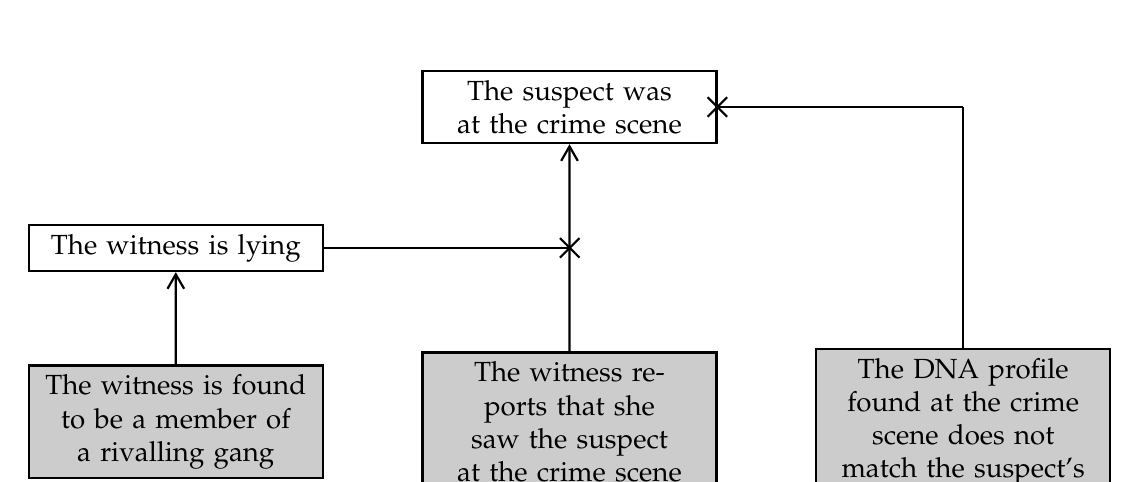
\begin{tikzpicture}[
		scnnode/.append style={text width=3cm},
		arg/.append style={text width=3.5cm},
	]
		\pgftransformxscale{5}
		\pgftransformyscale{2}

		% \draw[thick,dashed,rounded corners=1mm] (-1.45,0.45) rectangle (-0.55,-4.3);
		% \draw[thick,dashed,rounded corners=1mm] (-0.45,0.45) rectangle (0.
		% 45,-4.3);
		% \draw[thick,dashed,rounded corners=1mm] (0.55,0.45) rectangle (1.45,-4.3);

		\node[arg]     (conc) at (-1,0) {The suspect was at the crime scene};
%		\node[arg]     (oppconc) at (0,0) {The suspect was not at the crime scene};
		\node[arg,observed] (prem) at (-1,-2) {The witness reports that she saw the suspect at the crime scene};
		\node[arg,observed] (prem2) at (0,-2) {The DNA profile found at the crime scene does not match the suspect's};
		\node[arg,observed] (prem3) at (-2,-2) {The witness is found to be a member of a rivalling gang};

		\node[arg] (att) at ($(prem.north)!0.5!(conc.south)-(1,0)$) {The witness is lying};

		\draw[arg] (prem3) -- (att);
		\draw[] (prem2) -- (0,0);
		\draw[attack] (0,0) -- (conc);
		\draw[arg] (prem) -- (conc);
%		\draw[arg] (prem2) -- (oppconc);
%		\draw[attack] (prem2) -- (conc);
%		\draw[attack] (conc) -- (oppconc);
%		\draw[attack] (oppconc) -- (conc);
		\draw[attack] (att) -- ($(prem.north)!0.5!(conc.south)$);

	\end{tikzpicture}
\end{document}

\caption{Arguments with supporting and attacking reasons\label{fig:arg}}
\end{figure}


The analysis of the structure of arguments goes back to the early twentieth century when John Henry Wigmore developed his famous evidence charts~\citep{wigmore1913,wigmore1931}. The work by the New Evidence Scholarship~\citep{andersonEtal2005} continued from Wigmore's insights. Independently, and not focusing on evidence in criminal cases, the structure of arguments for and against conclusions was formalized and computationally studied by the philosopher John~\citet{pollock1987,pollock1995}. The work by Pollock stimulated an extensive literature on the formal and computational study of arguments for and against conclusions~\citep{vanEemerenEtal2014Ch11}.


\subsection{Probabilities}
\label{sec:normfram:prob}
The second normative framework %for the correct handling of the evidence 
uses probabilities as the main tool. 
In handling evidence in court, a crucial question from the probabilistic perspective is, 
how probable is a certain hypothesis $H$ given a body of evidence $E$? This is 
the \textit{conditional probability} of $H$ given $E$, or in symbols, $P(H|E)$. 
Another crucial question is, how does the probability of $H$ 
change in light of evidence $E$? This \textit{probability change} is expressed by 
the difference between the conditional probability $P(H|E)$ and the so-called \textit{prior 
probability} $P(H)$.
Both questions can be addressed with 
the famous Bayes' theorem:
%
\begin{quotation}
	$\Pr(H|E) = \dfrac{\Pr(E|H)}{\Pr(E)}\cdot\Pr(H)$
\end{quotation}
%
%<<<<<<< HEAD
%This formula---which can be easily proven from 
%the probability axioms---shows how the 
%conditional probability $\Pr(H|E)$ of hypothesis $H$ given evidence $E$ 
%can be computed by the prior probability $\Pr(H)$ and the 
%factor $\Pr(E|H)/\Pr(E)$. 
%\noindent One of the lessons of Bayes' theorem is that the more surprising 
%=======
This formula---which can be easily proven from 
the probability axioms\endnote{Bayes' theorem follows quickly using the definition of conditional probability. 
We have $\Pr(E|H) = \Pr(H\land E)/\Pr(H)$. Here we use logical conjunction $\land$ to write the combined event $H$ and $E$. 
Hence, $\Pr(H\land E)=\Pr(E|H)\cdot \Pr(H)$. It follows that
$\Pr(H|E) = \Pr(H \land E)/\Pr(E) = \Pr(E|H)\cdot \Pr(H)/\Pr(E)$, proving Bayes' theorem.
}---shows how the 
conditional probability $\Pr(H|E)$ of hypothesis $H$ given evidence $E$ 
can be computed by the prior probability $\Pr(H)$ and the 
factor $\Pr(E|H)/\Pr(E)$.  
%One of the lessons of Bayes' theorem is that the more surprising 
%>>>>>>> origin/master
%the evidence---that is, the lower $\Pr(E)$---the higher the probability 
%of the hypothesis given the evidence and the larger the probability increase. 
%To illustrate, compare two DNA profiles, one with a Random Match Probability of 1 in 10 and the other with 
%a Random Match Probability of 1 in 1 million. It is more surprising---that is, less probable---to find a match 
%for the latter than the former profile. Suppose now a genetic match is found between 
%the crime traces and a suspect. The hypothesis that the suspect is the source 
%of the traces is more probable (or the probability increase more pronounced) 
%if the matching profile has a lower Random Match Probability.

%To illustrate, suppose a trace is found at the crime scene 
%rare DNA profile of estimated frequency, or Random Match Probability, 1 in a billion. 
%and forensic analysis shows 
%that the suspect's DNA profile matches the crime trace. 
%Let $M$ be the match and $S$ the hypothesis that the suspect 
%is the source of the crime trace. The crucial questions, from a probabilistic standpoint, are: 
%How probable is the hypothesis $S$ given evidence $M$, that is, $P(S|M)$? And, 
%how does the evidence $M$ change the prior probability of $S$?
%In the sections that follow, we shall see to what extent these questions 
%can be addressed with the tools of probability. In particular, 
%we shall see how the probabilistic framework can take 
%into account the numerical part of DNA evidence, what we earlier described as the 
%Random Match Probability. 

%By Bayes' theorem, 
%
%\begin{quotation}
%	$\Pr(\neg S|M) = \dfrac{\Pr(M|\neg S)}{\Pr(M)}\cdot\Pr(\neg S)$
%\end{quotation}
%
%We cannot easily assign a number to the priopr probability 
%$\Pr(S)$ or Bayes' factor $\Pr(M|S)/\Pr(M)$ probabilities. Thus, 
%the value of $P(H|M)$ cannot be determined straightforwardly.  
%Still, we know the matching profile is rare; item Random Match 
%Probability is 1in a billion, so 
%
%\begin{quotation}
%	$\Pr(M) = 1/10^9$
%\end{quotation}
 %a match is not often found accidentally. 
%This statement can be made precise in the probability calculus. When $E$ expresses the evidence that the suspect's profile matches the trace's and $H$ that the suspect is not the source, we write:

%\noindent Here $\Pr(E|H)$ denotes the conditional probability that the suspect's profile matches the trace's, given the condition that the suspect is not the source. 
%noindent 
%MDB [THE TREATMENT OF BAYES THEOREM IS BRIEF AND IT'S UNCLEAR HOW IT IS CONNECTED WITH THE RANDOM MATCH PROBABILITY.]


The interest in probabilistic calculations as a tool for the good handling of the evidence has recently been stimulated by the statistics related to DNA profiling, and by some infamous miscarriages of justice that involved statistics, in particular the Lucia de Berk and Sally Clark cases~\citep{dawidEtal2011,fenton2011,schnepsColmez2013}. The interest is not new~\citep{tillers2011}, and can in fact be traced back to early forensic science in the late nineteenth century~\citep{taroniEtal1998}. To what extent probabilistic calculations have a place in courts has always been, and remains, the subject of debate.\endnote{A recent instance of the debate concerns the R v T case, where the UK Court of Appeal restricted the use of Bayes' theorem in courts to cases with a solid statistical foundation such as DNA; see the 2012 special issue of Law, Probability and Risk; Vol. 4, No. 2. For a 1970s instance of the debate, see~\citet{finkelsteinFairley1970,tribe1971}.}

\subsection{Scenarios}
\label{sec:introScen}
Finally, the third normative framework %for the correct handling of the evidence 
centers around scenario analysis. In a scenario, a coherent account of what may have happened in a case is made explicit. %Different scenarios are contrasted, and evaluated, by considering their plausibility and by checking to what extent they match and contradict the available evidence. 
Scenario analysis proves helpful when considering a complex case and its evidence. 
For instance, the following brief scenario can help to make sense of a murder case:
%
\begin{description}
	\item The robber killed the victim when caught during a robbery.	
\end{description}
%
\noindent Such a coherent explanation of the evidence in the form of
a scenario can be regarded as a sense-making tool for handling cases with a large dossier. 
%
%\begin{comment}
%For instance, consider a murder case in which a . An interpretation of what happened: 
%%with two suspects: the victim's former partner and a robber. For each suspect, a scenario is considered that explains the murder:
%
%\begin{description}
	%\item $S_1$: The victim's former partner killed the victim after a fight.
	%\item $S_2$: The robber killed the victim when caught during a robbery.	
%\end{description}

%When the robber confesses having killed the victim during a robbery, there is evidence contradicting scenario $S_1$ and matching scenario $S_2$.
%\end{comment}


Legal psychology has contributed to our knowledge about the role of scenarios in handling the evidence~\citep{bennettFeldman1981,penningtonHastie1993}. Scenarios were shown to be misleading, as experiments showed that a false scenario told in a sensible chronological order was more easily believed than a true scenario that was told in a random order. Still, the legal psychologists~\citet{wagenaarEtal1993} emphasised the usefulness of scenario analysis for the rational handling of the evidence, using the technique in their work on debunking dubious case decisions. Scenario analysis is connected with inference to the best explanation~\citep{pardoAllen2008}.

%MDB [I THINK WE SHOUD MAKE CLEAR THAT EACH FRAMEWORK WILL BE DEVELOPED MORE IN DEPTH LATER IN THE PAPER AND THAT IN THIS FIRST SECTION WE ARE  BEING GENERAL AND IMPRESSIONISTIC. THIS SECTIONS LOOKS LIKE A SUMMARY FO WHAT'S TO COME.]

\paragraph{Further readings} 
The three normative frameworks~\citep{andersonEtal2005,kapteinEtal2009,dawidEtal2011}. 

\textit{Arguments:} Wigmore charts~\citep{wigmore1913,wigmore1931}. The New Evidence Scholarship~\citep{andersonEtal2005}. 
Formal and computational study of arguments~\citep{pollock1987,pollock1995}.
Informal and formal argumentation theory~\citep{vanEemerenEtal2014}.

\textit{Probabilities:}
Evidence and probabilities~\cite{schum1994,morteraDawid2007}
Statistics in the law~\citep{fenton2011}. Miscarriages of justice involving statistics~\citep{dawidEtal2011,schnepsColmez2013}.
Debates on whether probabilistic calculations have a place in courts ~\citet{finkelsteinFairley1970,tribe1971}, back in 
1970's, and more recently, the 2012 special issue of \textit{Law, Probability and Risk}; Vol. 4, No. 2. 

\textit{Scenarios:}
Scenarios in evidential reasoning~\citep{bennettFeldman1981,penningtonHastie1993,penningtonHastie1993StoryModel}. Scenarios and miscarriages of justice~\citep{wagenaarEtal1993}. Inference to the best explanation~\citep{pardoAllen2008}. Hypothetical explanations of the evidence~\citep{thagard1989}. 


\textit{Combined approaches:}
Combining arguments and scenarios~\citep{bexEtal2010,bex2011}. Bayesian networks for evidential reasoning~\citep{heplerEtal2007,fentonNeilLagnado2013}. Combining arguments, scenarios and probabilities~\citep{vlekEtal2014, timmerEtAl2015ecsqaru, verheijEtal2016,verheij2014}.  

\section{Conflicting evidence}
\label{sec:conf}
 	
%\paragraph{Evidential reasoning in the law is a dialectical process involving reasons pro and con different reconstructions of the facts.} 

In many situations, it is clear what the facts are. In a simple case of tax evasion, for example, 
it will be easy to establish whether you filed for taxes on time and whether your employer paid you 100,000 dollars in 2015. Only in special circumstances, 
such as administrative errors, there will be something to dispute here. 
But cases that are litigated in court are typically more complicated.
Disputes emerge because the two parties---who then become the defense and the 
prosecution in a criminal trial---introduce evidence that support conflicting 
reconstructions of the facts. In this section, we illustrate how 
each of the three frameworks can represent and model conflicts 
between different pieces of evidence. 



%For example, a witness for the prosecutor may assert she saw the 
%defendant around the crime scene at the time of the crime, 
%while the defense may introduce evidence that the genetic material found 
%at the crime scene does not match the defendant's.


\subsection{Arguments}
\label{sec:confArg}


In the argument-based framework, the handling of conflicting evidence is analyzed 
in terms of arguments for and against a certain conclusion.


\paragraph{Three kinds of attack can be distinguished: rebutting, undercutting and undermining.}

Consider a crime case, where a witness testified she saw the suspect at the crime scene. The witness testimony constitutes a 
reason supporting the conclusion that the suspect indeed was at the crime scene. There are three parts to this argument: the conclusion; the reason (also called the premise); and the connection between the reason and the conclusion.
%More precisely, different kinds of attacking reasons can be distinguished. 
%Consider again the argument for the conclusion that the suspect was at the crime scene, supported by a witness reporting that she saw the suspect at the crime scene (Figure~\ref{fig:arg3}, on the left). 
Each of these three parts can be attacked. %This argument can be attacked in three ways. 

First, the conclusion can be attacked. %The suspect can for instance have an \textit{alibi}, 
%showing that he was not at the crime scene. 
For example, suppose DNA testing shows that the suspect does not genetically match 
with the traces found at the crime scene. 
Such an attacking reason is called a \textit{rebutting attack}.  
It supports the opposite conclusion, namely that the suspect was \textit{not} 
at the crime scene. 
%
Second, the reason itself can be attacked, although this is a bit more difficult to imagine.  
 For instance, %when the witness report is fraudulent, this is a reason for believing the witness did not report 
 if the witness never actually testified that she saw the suspect at the crime scene, this attacks the very 
 existence of the supporting reason itself. 
 %content of the witness testimony was misunderstood---for example, because the testimony was provided through a translation---this is a reason for 
 %doubting the witness actually testified she saw the suspect at the crime scene. 
 This kind of attack is referred to as \textit{undermining attack}. 
%
Third, the connection between the reason and the conclusion can be attacked.
 The fact that the lighting conditions were bad when the witness saw the crime, 
 is an example of such an attack, referred to as an \textit{undercutting attack}.
 % The lying of a witness is an example of such an attack, referred to as an \textit{undercutting attack}. 
 In contrast with a rebutting attack, an undercutting attack provides no support for the opposite conclusion. In the example, %when the witness is lying, 
 if the lighting conditions were bad, there is no reason explicitly 
 supporting that the suspect was not at the crime scene. The attacking reason, % statement, %here the lying of the witness, 
 here the bad lighting conditions, is also referred to as an exclusionary reason. 
%
The three examples of the different kinds of attack are shown in Figure~\ref{fig:arg3}.

\begin{figure}[bt]
\centering
\documentclass[border=5mm,tikz]{standalone} 

\usepackage{amsmath}
% !TEX root=img/arguments_and_attack.tex

% \usetikzlibrary{external} 
% \tikzexternalize[prefix=tikz/] 

\usetikzlibrary{calc}
\usetikzlibrary{arrows}
\usetikzlibrary{arrows.meta}
\usetikzlibrary{decorations.markings}
% \usetikzlibrary{intersections}
\usetikzlibrary{fit}
\usetikzlibrary{shapes}
% \usetikzlibrary{trees}


\tikzset{
	every path/.style={thick},
	align=center,
	observed/.style={
		fill=black!20,
	},
	bn/.style={
		draw,
		ellipse,
		-{Triangle[angle=60:6pt 0]}
	},
	scn/.style={
		draw,
		rectangle,
		% signal,
		% signal from=west,
		% signal pointer angle=120,
		-{Triangle[angle=60:6pt 0]},
	},
	possibly/.style={dashed},
	arg/.style={
		draw,
		rectangle,
		-{Straight Barb[angle=60:6pt 0]}
	},
	attack/.style={
		-{Rays[width=10pt,length=10pt,sep=-3.9pt]}
	},
	pref/.style={
		draw,
		rectangle,
		-{Straight Barb[angle=60:6pt 0]}
	},
	subscn/.style={
		double,
		-{Triangle[angle=60:6pt 0]},
	},
	specific/.style={
		double,
		-{Stealth[angle=60:6pt 0]}
	},
}



\begin{document}
	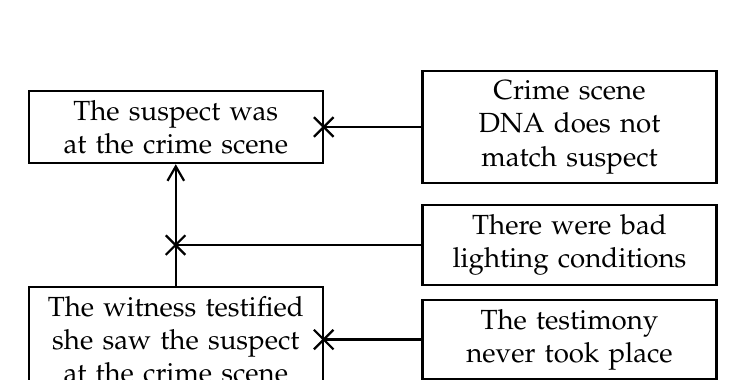
\begin{tikzpicture}[
		scnnode/.append style={text width=3cm},
		arg/.append style={text width=3.5cm},
	]
		\pgftransformxscale{5}
		\pgftransformyscale{2}

		\node[arg]     			(scene) at (0,-0.65) {The suspect was at the crime scene};
		\node[arg] (witn) at (0,-2) {The witness testified she saw the suspect at the crime scene};

		%\node[arg] 					(alibi) at (1,-0.65) {The suspect has an alibi}; 
		\node[arg] 					(alibi) at (1,-0.65) {Crime scene DNA does not match suspect}; 
		%\node[arg] 					(lying) at (1,-1.3) {The witness is lying};
		\node[arg] 					(lying) at (1,-1.4) {There were bad lighting conditions};
		\node[arg] 					(fraud) at (1,-2) {The testimony never took place};

		\draw[arg] 					(witn) -- (scene);

		\draw[attack] 			(alibi) -- (scene);
		\draw[attack] 			(lying) -- (0, -1.4);
		\draw[attack] 			(fraud) -- (witn);

	\end{tikzpicture}
\end{document}

\caption{Three kinds of attack\label{fig:arg3}}
\end{figure}

\paragraph{Three kinds of support can be distinguished: multiple, subordinated and coordinated.}

%I put attacking reasons first and then further supports second, because the further support seems a response to the there attacks

Just as attacking reasons can target the conclusion of an argument, its supporting
reason or the connection between the two, additional reasons 
can provide further support for each of these parts. %Having in mind a dialogical setting for analyzing the structure of arguments, 
Additional reasons can be seen as responses to attacking reasons or as reasons strengthening an existing argument. 

Consider, once again, the argument that the suspect was at the crime scene because the witness reports that she saw the suspect at the crime scene. 
First, the conclusion can be further supported, for example, by a second witness testimony. 
If a conclusion is supported by more than one reason, this is referred 
to as \textit{multiple support}. 
%
Second, the reason itself can be supported, for example, 
by a video recording of the witness testimony itself. 
Support of the reason itself is called \textit{subordinating support}. 
%MDB isn't this subordinating support simply a case of "chaining"
%
Finally, the connection between the reason and the conclusion can be further supported, for example, 
by another testimony that the witness has always been trustworthy and reliable. 
Support for the connection between the reason and the conclusion does not have a standard name, but is closely related 
to a third named kind of support: \textit{coordinated support}. In coordinated support, the support for the conclusion consists of at least 
two supporting reasons which, in their conjunctive combination, provide support for the conclusion. Coordinated support is distinguished from multiple support because in the latter each supporting reason 
provides support for the conclusion by itself. 
%
Figure~\ref{fig:support} shows the three kinds of (further) support. (Multiple and subordinated support are graphically visualized with an arrow, whereas coordinated support is shown with a line. An arrow indicates the unnamed kind of support of the connection between reason and conclusion.)

\begin{figure}[bt]
\centering
\documentclass[border=5mm,tikz]{standalone} 

\usepackage{amsmath}
% !TEX root=img/arguments_and_attack.tex

% \usetikzlibrary{external} 
% \tikzexternalize[prefix=tikz/] 

\usetikzlibrary{calc}
\usetikzlibrary{arrows}
\usetikzlibrary{arrows.meta}
\usetikzlibrary{decorations.markings}
% \usetikzlibrary{intersections}
\usetikzlibrary{fit}
\usetikzlibrary{shapes}
% \usetikzlibrary{trees}


\tikzset{
	every path/.style={thick},
	align=center,
	observed/.style={
		fill=black!20,
	},
	bn/.style={
		draw,
		ellipse,
		-{Triangle[angle=60:6pt 0]}
	},
	scn/.style={
		draw,
		rectangle,
		% signal,
		% signal from=west,
		% signal pointer angle=120,
		-{Triangle[angle=60:6pt 0]},
	},
	possibly/.style={dashed},
	arg/.style={
		draw,
		rectangle,
		-{Straight Barb[angle=60:6pt 0]}
	},
	attack/.style={
		-{Rays[width=10pt,length=10pt,sep=-3.9pt]}
	},
	pref/.style={
		draw,
		rectangle,
		-{Straight Barb[angle=60:6pt 0]}
	},
	subscn/.style={
		double,
		-{Triangle[angle=60:6pt 0]},
	},
	specific/.style={
		double,
		-{Stealth[angle=60:6pt 0]}
	},
}



\begin{document}
	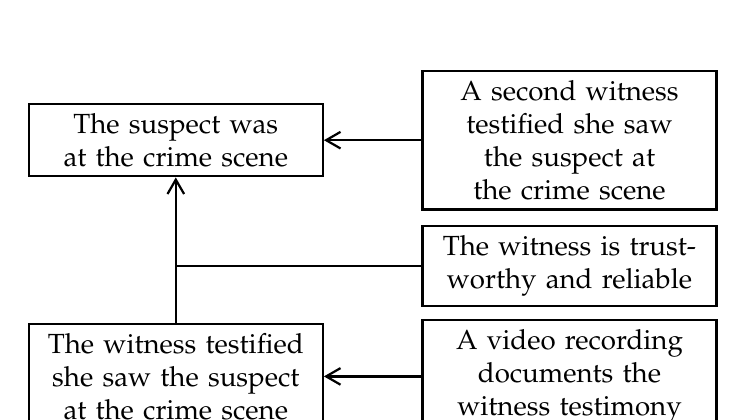
\begin{tikzpicture}[
		scnnode/.append style={text width=3cm},
		arg/.append style={text width=3.5cm},
	]
		\pgftransformxscale{5}
		\pgftransformyscale{2}

		\node[arg]     			(scene) at (0,-0.5) {The suspect was at the crime scene};
		\node[arg] 					(witn) at (0,-2) {The witness testified she saw the suspect at the crime scene};

		\node[arg] 					(alibi) at (1,-0.5) {A second witness testified she saw the suspect at the crime scene};
		\node[arg] 					(lying) at (1,-1.3) {The witness is trustworthy and reliable};
		\node[arg] 					(fraud) at (1,-2) {A video recording documents the witness testimony};

		\draw[arg] 					(witn) -- (scene);

		\draw[arg] 			(alibi) -- (scene);
		\draw 					(lying) -- (0, -1.3);
		\draw[arg] 			(fraud) -- (witn);

%%%

		%\node[arg]     			(scene) at (1.85,-0.5) {The suspect was at the crime scene};
		%\node[arg] 					(witn) at (1.85,-2) {The witness reports that she saw the suspect at the crime scene};
%
		%\node[arg] 					(lying) at (2.35,-1.15) {The witness report is trustworthy};
%
		%\draw[arg] 					(witn) -- (scene);
%
		%\draw 					(lying) -- (1.85, -1.15);




	\end{tikzpicture}
\end{document}

\caption{Three kinds of (further) support\label{fig:support}}
\end{figure}

%MDB INTERESTING DISTINCTIONS BUT THE TERMINOLOGY IS HEAVY AND SOMEWHAT CONFUSING. CAN WE MAKE THIS SHORTER?

%\paragraph{The arguments for and against different positions have structure, involving complexes of reasons supporting and attacking positions.}  MDB changed
\paragraph{Arguments have structures, involving complexes of supporting and attacking reasons.} 

So far we have looked at a simple argument,  consisting of a reason and a conclusion, along with three types 
of attacking reasons and three types of symmetric supporting reasons. But an argument can also be more complex, 
for example, it can contain \textit{chains of reasons}. 

Consider, once again, the example of a witness who reports that she saw the suspect at the crime scene. The witness testimony constitutes a 
reason supporting the conclusion that the suspect was at the crime scene, and this conclusion---in turn---functions as a reason 
that supports the conclusion that the suspect committed the crime. This chain of supporting reasons 
is graphically depicted in Figure~\ref{fig:arg2}, on the left. 
Attacking reasons can also be chained. For example, when it is discovered that the witness is a member of a rivaling gang, 
this constitutes a reason for concluding that the witness has an interest in lying, and further, for concluding 
that the witness is in fact lying (Figure~\ref{fig:arg2}, on the right). This conclusion attacks---undercuts, to be precise---the connection 
between the witness testimony and the conclusion the suspect was at the crime scene.

\begin{figure}[bt]
\centering
\documentclass[border=5mm,tikz]{standalone} 

\usepackage{amsmath}
% !TEX root=img/arguments_and_attack.tex

% \usetikzlibrary{external} 
% \tikzexternalize[prefix=tikz/] 

\usetikzlibrary{calc}
\usetikzlibrary{arrows}
\usetikzlibrary{arrows.meta}
\usetikzlibrary{decorations.markings}
% \usetikzlibrary{intersections}
\usetikzlibrary{fit}
\usetikzlibrary{shapes}
% \usetikzlibrary{trees}


\tikzset{
	every path/.style={thick},
	align=center,
	observed/.style={
		fill=black!20,
	},
	bn/.style={
		draw,
		ellipse,
		-{Triangle[angle=60:6pt 0]}
	},
	scn/.style={
		draw,
		rectangle,
		% signal,
		% signal from=west,
		% signal pointer angle=120,
		-{Triangle[angle=60:6pt 0]},
	},
	possibly/.style={dashed},
	arg/.style={
		draw,
		rectangle,
		-{Straight Barb[angle=60:6pt 0]}
	},
	attack/.style={
		-{Rays[width=10pt,length=10pt,sep=-3.9pt]}
	},
	pref/.style={
		draw,
		rectangle,
		-{Straight Barb[angle=60:6pt 0]}
	},
	subscn/.style={
		double,
		-{Triangle[angle=60:6pt 0]},
	},
	specific/.style={
		double,
		-{Stealth[angle=60:6pt 0]}
	},
}



\begin{document}
	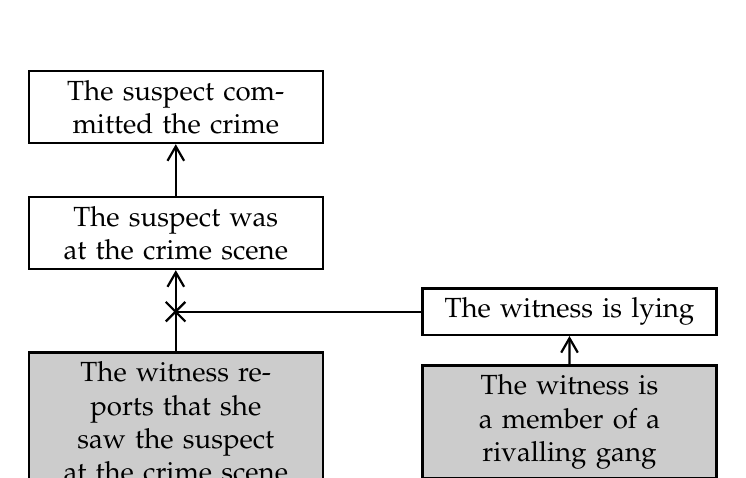
\begin{tikzpicture}[
		scnnode/.append style={text width=3cm},
		arg/.append style={text width=3.5cm},
	]
		\pgftransformxscale{5}
		\pgftransformyscale{2}

		\node[arg]     			(comm) at (0,0) {The suspect committed the crime};
		\node[arg]     			(scene) at (0,-0.8) {The suspect was at the crime scene};
		\node[arg,observed] (witn) at (0,-2) {The witness reports that she saw the suspect at the crime scene};

		\draw[arg] 					(witn) -- (scene);
		\draw[arg] 					(scene) -- (comm);

		\node[arg] 					(lying) at (1,-1.3) {The witness is lying};
		\node[arg,observed] (rival) at (1,-2) {The witness is a member of a rivalling gang};

		\draw[attack] 			(lying) -- (0, -1.3);
		\draw[arg] 					(rival) -- (lying);

	\end{tikzpicture}
\end{document}

\caption{Supporting and attacking reasons can be chained. \label{fig:arg2}}
\end{figure}





%\paragraph{In an argumentative dialogue, parties take positions supported by reasons that can be challenged by attacking reasons.}
%
%Arguments have a dialogical counterpart, in which parties exchange reasons for and against the positions they endorse. The arguments shown in Figure~\ref{fig:arg2} for instance form the backbone of the following argumentative dialogue---here presented as a fictitious, stylized discussion between judge, prosecution and defense:
%
%\begin{description}
	%\item \emph{Prosecution}: The suspect committed the crime.
	%\item \emph{Judge}: Why do you believe that?
	%\item \emph{Prosecution}: The suspect was at the crime scene.
	%\item \emph{Judge}: Do you have evidence supporting that position?
	%\item \emph{Prosecution}: There is a witness reporting that she saw the suspect at the crime scene.
	%\item \emph{Defense}: Objection, your honor! The witness is lying.
	%\item \emph{Judge}: Why do you believe that?
	%\item \emph{Defense}: The witness is a member of a rivalling gang.
%\end{description}
%
%
%
%[I LIKE VERY MUCH THE DESCRIPTION OF THE THREE KINDS OF ATTACKS AND THE GRAPHICAL ILLUSTRATION. BUT THIS PART ABOUT THE DIALOGUE IS STRANGE. 
%FIRST, THE DIALOGUE IS UNNATURAL. SECOND, I AM NOT SURE THIS IS ABOUT ARGUMENTS ANYMORE. ARGUMENTS CAN COME IN THE FORM OF A DIALOGUE 
%BUT  NEED NOT BE. PERHAPS WE NEED TO REDEFINE THE ARGUMENT FRAMEWORK AS DIALOGUE/ARGUMENT FRAMEWORK?]
%
%\noindent Models of argumentative dialogue involve specifications of the kinds of moves parties can make, the commitments these moves imply for parties, and the rules that determine the allowed sequences of dialogue moves.

\paragraph{Further readings} 
Argument structure and diagrams~\citep{wigmore1913,wigmore1931,toulmin1958,freeman1991}. Defeasible reasoning and nonmonotonic logic~\citep{pollock1987,gabbayEtal1994}. Rebutting and undercutting attack~\citep{pollock1987,pollock1995}. Undermining attack~\citep{bondarenkoEtal1997}. Formal evaluation of defeasible arguments~\citep{pollock1987,pollock1995,dung1995,prakken2010}. Argumentative dialogue~\citep{toulmin1958,waltonKrabbe1995,prakken1997,hage2000}. Accrual of reasons and weighing~\citep{pollock1995,hage1997,verheij1996diss,prakken2005}. Argument diagramming and evaluation software~\citep{pollock1995,reedRowe2004,kirschnerEtal2003,vanGelder2003,verheij2005,gordonEtal2007}.

\subsection{Scenarios}

In the scenarios normative framework, the handling of conflicting evidence is analyzed by considering different scenarios about what may have happened.

\paragraph{There may be conflicting scenarios about what has happened.} 
The prosecution and the defense often 
present different scenarios about what happened. For example, 
in a murder case, the parties may put forward two scenarios, as follows:

\begin{description}
	\item $S_1$: The defendant killed the victim when caught during a robbery.
	\item $S_2$: The defendant was at home with his wife.	
\end{description}

\noindent The former is a robbery scenario, and the latter an \textit{alibi} scenario. They are conflicting since 
only one of them can be true. Note that the second scenario does not say who killed the victim or how the crime occurred. 
It only asserts that the defendant did not do it.
%Here the conflict is connected to the different sides, prosecution and defence. 
But there can also be conflicting scenarios, each pointing to a different perpetrator:

\begin{description}
	\item $S_1$: The defendant killed the victim when caught during a robbery.
	\item $S_3$: The victim's former partner killed the victim after a violent fight between the two.
\end{description}
%
The two scenarios offer incompatible reconstructions of how the killing 
occurred and who did it, because they cannot be both true. 

\paragraph{Evidence can be explained by one scenario, but not by another.} 
Conflicts between scenarios can also exist in relation to the evidence, for example, when one scenario 
can explain a piece of evidence but the other cannot.  Two senses of `explanation' are relevant here. First, 
a scenario explains the evidence in the sense that it \textit{predicts} the evidence. 
There is another, albeit closely related, sense of explanation.  
A scenario explains the evidence in the sense that it exhibits the \textit{causal process} by which the evidence 
was brought about. 

%This applies most naturally to physical and testimonial evidence. 
%In a case in which traces were found at the crime scene, 
%it is more plausible that an individual visited the crime scene 
%and left the traces by physical contact.

Consider, for example, the conflicting scenarios $S_1$ and $S_3$.
%Both scenarios explain the starting point of the murder investigation: the victim's body found at the crime scene (evidence $E_2$), in the sense that finding the body is expected assuming either scenario to be true. 
Suppose now that laboratory analyses find a genetic match between the DNA profile of a tissue trace found under 
the victim's fingernails and his former partner. Scenario $S_3$ can explain the presence of the matching trace. The explanation is that the victim's former partner is the 
source of the trace, which was deposited during the violent fight between the two. The scenario can predict 
the presence of the trace, in the sense that if the scenario is assumed to be true, the matching trace must be there or 
likely to be there. The scenario also exhibit the causal process that brought about the trace, namely the violent fight, altercation 
and physical contact between the two.  Scenario $S_1$, the robbery scenario, cannot explain the presence of the trace matching the victim's former partner. 
However, suppose another piece of evidence 
is that the victim's house was in fact robbed. Scenario $S_1$ can explain this evidence, but not $S_3$. All in all, scenarios $S_1$ and $S_3$ 
are not only inconsistent on their face, they also diverge
in terms of the evidence that they can or cannot explain.

\paragraph{Scenarios can be contradicted by evidence.} So far we considered scenarios that are 
inconsistent with one other because 
they cannot be both true, but also scenarios that diverge in terms of 
the evidence they can or cannot explain. There is another type of conflict worth discussing. This takes the form of 
a quasi-inconsistency between scenarios and  evidence. The quasi-inconsistency occurs when the evidence, 
typically testimonial, not physical or trace evidence, asserts that such-and-such occurred, while the scenario 
denies it. 

%Just as there can be conflict between scenarios considered \textit{per se}, 
%there can be conflicts between scenarios and the evidence presented. 
Suppose a video recording shows the suspect 
breaking into the victim's house, and upon being discovered, 
killing the victim and later stealing the jewelry. 
This evidence contradicts the alibi scenario $S_2$ but also scenario $S_3$ 
in which the victim's former partner is the killer.  More carefully, insofar as the evidence 
is taken at face value---that is, the video is taken to be a truthful representation---scenario $S_2$ and $S_3$ 
are inconsistent with the evidence, while scenario $S_1$ is consistent. 

\begin{comment}
Let's consider a murder case with two alternative scenarios: a former partner murder scenario $S_1$ where the victim's former partner murders the victim, and a robbery murder scenario $S_2$ where a robber murders the victim when caught during a robbery. If the robber's partner presents an alibi (evidence $E_1$), this evidence contradicts scenario $S_2$. 
This evidence is independent from scenario $S_1$.
\end{comment}


\begin{comment}
%By assuming the truth of the scenario, the presence of the evidence can be derived more or less deductively. 
This can expressed by the statement \textit{if} $S$, \textit{then} $e$, 
where $S$ is a scenario and $e$ the evidence, in the sense that $e$ 
follows deductively from $S$. The relation of prediction can also be probabilistic, in the sense that given the truth of the scenario, 
the truth of the evidence is highly probable. 
%In the language of probability, the conditional probability $P(E|H)$ of $e$ given $S$ can also be used, where the higher the probability, the better 
%the scenario's predictive power relative to the evidence. 
For example, let $V$ be a scenario that comprises the event that the defendant visited the crime scene, and let $M$ be 
evidence that certain genetic material matching the defendant 
was found at the crime scene. Clear $V$ predicts $M$, in the sense that from the truth of $V$
 the match $M$ follows almost deductively or at least with a high probability.  
%If a scenario can predict the evidence, this fact favors the scenario, and if it cannot, this weakens the credibility of the scenario.

There is another sense of explanation that deserves mentioning here. 
A scenario explains the evidence in the sense it exhibits the \textit{causal process} by which the evidence 
was brought about. This applies most naturally to physical and testimonial evidence. 
In a case in which traces were found at the crime scene, 
it is more plausible that an individual visited the crime scene 
and left the traces by physical contact. Here the scenario exhibits the causal process (physical contact) 
by which the existence of the evidence 
(traces) was brought about. 
\end{comment}

\paragraph{Further readings} 
Scenarios in evidential reasoning~\citep{bennettFeldman1981,penningtonHastie1993,penningtonHastie1993StoryModel}. Scenarios and miscarriages of justice~\citep{wagenaarEtal1993}. Inference to the best explanation~\citep{pardoAllen2008}. Hypothetical explanations of the evidence~\citep{thagard1989}. 

\subsection{Probabilities}

In the probabilistic normative framework, the handling of conflicting evidence is analyzed in terms of the conditional probabilities that connect the evidence and the hypotheses.

\paragraph{Evidential support and attack can be characterized as ``probability change''.} 
%BV:I changed difference to relevance, as 'prob diff' is used later for something else.
%BV:I prefer replacing 'favoring and disfavoring' by 'suport ad attack', throughout. MDB: DONE
%MDB : used the expression "probability changes" because relevant is general and might apply also to a likelihood ratio greater than one. 
A piece of evidence $E$ supports an 
hypothesis $H$ whenever $E$ raises the probability of $H$, or in symbols, 
$P(H|E) > P(H)$. 
For example, a witness 
testifies that she saw the defendant around the crime scene
 at the time of the crime. The testimony supports the hypothesis 
 that the defendant is guilty. 
This can be described probabilistically, as follows:
 %
 \[ P(\textit{guilt}|\textit{testimony}) > P(\textit{guilt}).\] 
 %
By contrast, a piece of evidence $E$ attacks a hypothesis $H$ whenever $E$ lowers 
the probability of $H$, or in symbols, $P(H|E) < P(H)$.
For example, if a DNA test shows no match between the traces found at the crime
 scene and the defendant, this evidence attacks the hypothesis that the defendant is guilty. 
 Probabilistically, 
%
\[ P(\textit{guilt}|\textit{no DNA match}) < P(\textit{guilt}).\]  
%
 %
 
% \paragraph{Two characterizations of evidential favoring and disfavoring are equivalent} 
\paragraph{Evidential support and attack can be characterized as ``likelihood ratio''.} 

There is another characterization of evidential support and attack. 
Instead of comparing the initial probability $P(H)$ and the probability $P(H|E)$ 
of the hypothesis given the evidence, a so-called likelihood ratio of 
the form ${P(E| H)}/{P(E |\neg H)}$ 
%BV: I changed the vertical fraction to a horizontal one. Looks better inline. I prefer that everywhere.
can also be used.
On this account, $E$ supports $H$ whenever the likelihood ratio
$\frac{P(E|H)}{P(E | \neg H)}$ is greater than one. Intuitively, this means that the presence of the 
evidence is more probable %BV was 'likely'
if the hypothesis is true than if the hypothesis is false. 
By contrast, a piece of evidence $E$ attacks a hypothesis $H$ whenever 
the likelihood ratio is lower than one. This means that the presence of the evidence is less likely %BV was 'likely'
if the 
hypothesis is true than if the hypothesis is false. For the two examples considered earlier, we have:
%
 \[\frac{P(\textit{testimony}|\textit{guilt})}{P(\textit{testimony}|\neg \textit{guilt})} > 1, \text{ and }\]
 %
 \[\frac{P(\textit{no DNA match}|\textit{guilt})}{P(\textit{no DNA match}|\neg \textit{guilt})} < 1.\]
%
These two characterizations of evidential support/attack---in terms of probability 
increase/decrease, and in terms of a likelihood ratio greater/lower than one---are 
in fact equivalent. 
For the following statements hold:
%
%\[\textit{\text{$E$ favors (or supports) $H$} iff }   P(H|E)> P(H) \textit{ iff }\frac{P(E|H)}{P(E|\neg H)}>1.\]
\[ P(H|E)> P(H) \text{ iff }\frac{P(E|H)}{P(E|\neg H)}>1.\endnote{To see why, recall that 
%
\[ \frac{P(H|E)}{P(\neg H | E)} = \frac{P(E | H)}{P(E| \neg H)}\cdot \frac{P(H)}{P(\neg H)},\]
%
%BV The LR formula should be in the main text somewhere
%BV I like having this proof. (Source?)
%BV I don't like a long, complex footnote. Let's discuss.
which implies
%
\[\frac{P(E|H)}{P(E|\neg H)}>1 \text{ iff } \frac{P(H|E)}{P(\neg H | E)} > \frac{P(H)}{P(\neg H)}.\]
%
For one direction, if $P(H|E)> P(H)$, then $1- P(H|E)< 1- P(H)$. This means that 
$\frac{P(H|E)}{1- P(H | E)} > \frac{P(H)}{1- P(H)}$, and thus
$\frac{P(H|E)}{P(\neg H | E)} > \frac{P(H)}{P(\neg H)}$. So, by the equivalence above, $\frac{P(E|H)}{P(E|\neg H)}>1$.
For the other direction, if $\frac{P(E|H)}{P(E|\neg H)}>1$, then $\frac{P(H|E)}{P(\neg H | E)} > \frac{P(H)}{P(\neg H)}$, again 
by the equivalence above. 
The latter is the same as $\frac{P(H|E)}{1- P(H | E)} > \frac{P(H)}{1- P(H)}$. To establish $P(H|E)> P(H)$, suppose for contradiction that
$P(H|E) \leq P(H)$, which implies $1- P(H|E) \geq 1- P(H)$. This means that $\frac{P(H|E)}{1- P(H | E)} \leq \frac{P(H)}{1- P(H)}$. 
This contradicts $\frac{P(H|E)}{1- P(H | E)} > \frac{P(H)}{1- P(H)}$, and thus $P(H|E)> P(H)$.}\]
 %
\[ P(H|E) < P(H) \text{ iff}  \frac{P(E|H)}{P(E|\neg H)} < 1.\]
%

\paragraph{The conflict between two pieces of evidence can be described probabilistically.}
Two pieces of evidence come into 
conflict with one another insofar as one supports a hypothesis 
and the other attacks the same hypothesis. 
The conflict can be described probabilistically, in that one piece of evidence increases 
the probability of the hypothesis, while the other decreases it, or equivalently, the likelihood ratio is positive (for one piece 
of evidence) and negative (for the other). 
For example, the testimony that the defendant was around the crime scene conflicts 
with the lack of a DNA match. Probabilistically, the testimony 
increases the probability of the defendant's guilt (or equivalently, the likelihood ratio is greater than one),
while the lack of a DNA match decreases the probability of the same hypothesis 
(or equivalently, the likelihood ratio is lower than one).
%BV Nothing is said about conflict resolution. 

\paragraph{Further readings} 
%.........................................................................................
On confirmation theory and accounts of evidential support \citep{carnap1950, fitelson1999, crupi2015}.

\section{Evidential value}
\label{sec:str}

The evidence found in a criminal investigation has different levels of evidential value: some evidence is very strong, other not so much. How is evidential value handled in each of the three normative frameworks? That is the topic of this section.

\subsection{Probability}

In the probabilistic framework, evidential value is measured using the numeric calculus of probability theory.

	
%\paragraph{The evidential value of a piece of evidence is measured by probabilistic difference or likelihood ratio (`incremental evidential value').}

\paragraph{The incremental evidential value is measured by the probabilistic difference.}
%BV Some reshaping is needed in this section, I'd say. 1. There is the evidential value of a piece of evidence; measured by probabilistic difference or LR (`incremental evidential value'). 2. There is the evidential value of all the evidence, in its totality; measured by the overall conditional prob (`total evidential value'). 3. DNA evidence is a good example, but there are complications.
%BV Below the discussion of the drunk witness is (for me) a complicated way of saying that a drunk witness has (by itself) hardly incremental evidential value. What is the lesson to be taught?
%BV In the part on DNA evidence I'd also reshape. For me the RMP connects a match (an actual match, M) probabilistically with the suspect being the source (S); we did that in the project paper verheijEtal2016. I'd first like to see that discussed, and then explained that there also are complications. Here the so-called hierarchy of propositions should be mentioned. cookEtAl1998, evettEtal2000 if I am correct.
The incremental value of evidence for, or against, a hypothesis 
can be quantified probabilistically in various ways. 
%The probabilistic framework allows us to quantify the strength of the evidential favoring or support relation between evidence and hypothesis. 
%The are different approaches in the literature. % (FITELSON REFERENCE HERE). 
%Let us begin with quantifying the value of the evidence \textit{for} an hypothesis. 
One approach considers the difference between the probability of 
the hypothesis with and without the evidence, that is, $P(H | E) - P(H)$.
%If $P(H | E)$ is higher than $P(H)$, this means that the evidence lends some support to
%the hypothesis. 
The larger the positive difference, the higher the value of the evidence 
for the hypothesis. 
%By contrast, the larger the negative difference, the higher the value of the evidence against the hypothesis. 
An alternative approach is given by the likelihood ratio $P(E|H)/P(E| \neg H)$. 
%For the evidence to offer some support to the hypothesis, the likelihood ratio should be at least greater than one. 
For any value greater than one, the higher the likelihood ratio, 
the higher the value of the evidence for the hypothesis. %For simplicity, we shall speak of evidential strength 
%in terms of likelihood ratios, as follows:
%
%\begin{quote}
%\textsc{Evidential strength:} The evidential strength of $E$ relative to $H$ is proportional to 
%the likelihood ratio $\frac{P(H|E)}{P(H|\neg E)}$. 
%\end{quote}
%
%By contrast, for any value lower than one, the lower the likelihood ratio 
%the higher value of the evidence against the hypothesis. 
\begin{comment} 
The following table %, whose calculations are approximations based on Bayes' theorem, offers 
offers some illustrations:

\vspace{2mm}
\hspace{0.5cm}
\begin{centering}
\begin{tabular}{lccccc}
\hline
$P(H)$ & Likelihood Ratio & $P(H | E)$ &  $P(H|E)-P(H)$ \\
\hline
0.0001 & 1,000 & 0.09 &  0.0899   \\
%0.001 & 1,000 & 0.049 & 0.5  \\
%0.01  & 1,000 & 0.08  & 0.9 \\
0.1 & 1,000  & 0.99 &  0.89 \\
\hline
%0.5 & 1,000 &   0.999 \\
%0.9 & 1,000 &   0.9999 \\
0.0001 & 10  & 0.001 &  0.0009 \\
0.01 & 10  & 0.09 &  0.08  \\
\hline
\end{tabular}
\end{centering}
\vspace{2mm}

\noindent
%Note that even if the likelihood ratio is high, the probability $P(G|E)$ can 
%still be low if the initial probability $P(H)$ is itself low. 
All in all, a positive difference $P(H|E) - P(H)$ and a likelihood ratio ${P(E|H)}/{P(E| \neg H)}$ greater than one
%tell us how much a piece of evidence $E$ can impact upwards the initial 
%probability of a hypothesis $H$. They 
quantify, albeit in different ways, the value of the evidence \textit{for} 
a hypothesis. 
\end{comment}
 By contrast, a negative difference $P(H | E) - P(H)$ and a likelihood ratio lower than one  
quantify the value of the evidence \textit{against} a hypothesis.
The larger the negative difference and the lower the likelihood ratio (for any value below one), 
the higher the value of the evidence against the hypothesis.

%As one can see from the table, there are quantitive 
%differences between the two approaches, but these should 
%not concern us here. Since the most widely used approach to quantify evidential value relies on 
%likelihood ratios, we shall use that, making occasional 
%references to the other approach if necessary. 

%\paragraph{The overall probability is not the same as probability difference and likelihood ratio}

%\paragraph{The evidential value of all the evidence, in its totality, is measured by the overall conditional probability (`overall evidential value'). }

\paragraph{The overall evidential value is measured by the overall conditional probability. }

In contrast with the incremental evidential value of evidence that is measured by a probabilistic difference or likelihood ratio, the overall evidential value of the full body of evidence is measured by the conditional probability 
of the hypothesis given the evidence. The higher, or lower, the probability $P(H|E)$, the higher 
the overall value of the evidence for, or against, the hypothesis. If there is a series of pieces of evidence $E_1, \ldots, E_n$, the overall evidential value of the evidence is measured as $P(H|E_1, \ldots, E_n)$.

Overall and incremental evidential value should not be confused. To illustrate, suppose we have strong evidence $E_1$ for the hypothesis $H$ 
that a suspect was at the crime scene, for instance, security camera footage in which the suspect is easily recognizable. 
In this case, the overall evidential value $P(H|E_1)$ of the evidence is high. If this is the only evidence, then also the 
incremental evidential value is high: before the evidence is considered, the hypothesis is not strongly supported, i.e.\ $P(H)$ is low, whereas after the evidence is considred, 
the hypothesis is strongly supported, i.e.\ $P(H|E_1)$ is high. In this case, the overall and incremental evidential value of $E_1$ are both high. 
But suppose a witness testifies that the defendant was not at the crime scene (evidence $E_2$), but as it turns out, the witness is unreliable 
as a known accomplice of the suspect. Consider now the overall evidential value $P(H|E_1, E_2)$ of the two pieces of evidence together. This will not have changed much when compared to $P(H|E_1)$. As a result, the incremental evidential value of $E_2$ is low, while still the overall evidential value $P(H|E_1, E_2)$ is high, even though $E_2$ did not contribute much. 

The difference between overall and incremental evidential value can be especially confusing when there is a single piece of evidence and there is a misalignment between the two values. Consider the hypothesis $\neg H$ that the suspect was not at the crime scene and the evidence $E_2$, the testimony of the unreliable witness. Then $P(\neg H)$ is high and also $P(\neg H | E_2)$ is high. Uncritically interpreted, the high value of $P(\neg H | E_2)$ suggests that the testimony of the unreliable witness has a high evidential value. But incrementally $E_2$ did not change much. The hypothesis $\neg H$ is, in totality, still strongly supported after the incrementally weak evidence $E_2$, since the hypothesis was already strongly supported before that evidence. 

%In this case, the incremental evidential value of the testimony in favor of guilt can be regarded as slightly incriminating. Hence we expect the probabilistic difference $P(\textit{guilt} | \textit{drunk witness})$ to be a small positive value, and the likelihood ratio $P(\textit{guilt} | \textit{drunk witness})/P(\textit{guilt} | \neg\textit{drunk witness})$ to be slightly above one.
%
%Now assume that the testimony by the drunk witness is the only incriminating evidence. In this case, 
%
%
%, the probability 
%$P(\textit{guilt} | \textit{drunk witness})$ should also be low. Now, it follows that $P(\textit{innocence} | \textit{drunk witness})$ 
%should be high insofar as \textit{innocence} is the negation of \textit{guilt}. 
%But this seems problematic. A drunk witness, in fact, is of little help in establishing 
%innocence (just as it is of little help in establishing guilt).
%
%It is instructive to quantify the value of the testimony in favor of guilt by means of 
%the probability difference and the likelihood ratio. Since the witness was drunk, the value of the evidence in favor of guilt is 
%low, that is:
%%
%\[\text{the positive difference $P(\textit{guilt} | \textit{drunk witness}) - P(\textit{guilt})$ is small, and}\]
%%
%%
%\[\text{the likelihood ratio $\frac{P(\textit{guilt} | \textit{drunk witness})}{P(\textit{guilt} | \neg\textit{drunk witness})}$ is only slightly above one}.\] 
%%
%Similarly, the value of the evidence in favor of innocence is also low, that is:
%%
%\[\text{the negative difference $P(\textit{innocence} | \textit{drunk witness}) - P(\textit{guilt})$ is small, and}\]
%%
%%
%\[\text{the likelihood ratio $\frac{P(\textit{innocence} | \textit{drunk witness})}{P(\textit{innocence} | \neg\textit{drunk witness})}$ is only slightly below one}.\] 
%%
%So, the value of the testimony in favor of guilt, and innocence, is low 
%in both cases. This means that $P(\textit{guilt} | \textit{drunk witness})$
%and $P(\textit{guilt})$ are roughly the same value, and so are $P(\textit{innocence} | \textit{drunk witness})$ 
%and $P(\textit{innocence})$. Consequently, if $P(\textit{innocence})$ is high, 
%and thus $P(\textit{guilt})$ low, $P(\textit{innocence} | \textit{drunk witness})$ will 
%be high, and thus $P(\textit{guilt} | \textit{drunk witness})$ low. %, given the little evidential value of the testimony. 
%We should thus not be surprised that $P(\textit{innocence} | \textit{drunk witness})$ is high. 
%This is because, by Bayes' theorem, $P(H|E)$ depends on $P(H)$.  
%Even if $E$ does not change significantly the probability of $H$, or the likelihood ratio (positive or negative) 
%$\frac{P(E|H)}{P(E| \neg H)}$ is small, $P(H|E)$ could still be high or low, insofar as $P(H)$ itself is high or low. 
%All in all, we should be careful in not confusing a high probability $P(H|E)$ with a high 
%evidential value in terms of a large probability difference or a high likelihood ratio.


\paragraph{DNA evidence has high incremental evidential value, but there are complications.}

%A widely used measure of evidential value 
%is the likelihood ratio. 
As an illustration, we discuss the likelihood ratio 
of a DNA match. %, where the match is between
%the crime scene's genetic profile and the defendant's. 
%Suppose the DNA test reports a match between the crime traces and the defendant.  %Given our simplifying assumptions, 
When introduced in court, a DNA match comes with an 
estimated Random Match Probability (RMP).  One way to interpret this probability is 
as the probability that a random person, who 
had nothing to do with the crime, would match. %An RMP is derived from the estimated frequency of the DNA profile across a sample population. 
%We should bear in mind that genetic profiles are not unique. 
%Based on statistical and genetic modeling,  a profile is expected to occur 
%with a  certainfrequency in a select population. 
%
Now, with some simplifications (on these later), 
the evidential value of the DNA 
match $M$ in favor of the suspect being the source of the sample $S$, in terms of a likelihood ratio, 
is as follows % \citep{Dawid02, Balding2005Weight}:
%
\[
\frac{P(M | S)}{P(M | \neg S)} =   \frac{1}{RMP}.
\]
%
%BV RMP is as yet undefined
The numerator $P(M | S)$ equals 1 because we assume that %of our simplifying assumption that 'source' and guilt' are interchangeable 
%and the laboratory test is infallible. If 
if the defendant is the source of the sample%and thus the source of the crime traces
, the lab test will report a match. As for the denominator, 
%keep in mind that $RMP$ is the probability that a random person, 
%unrelated to the crime or the defendant, would be found to have a matching DNA. 
putting $P(M | \neg S)=RMP$ is plausible because the probability that a match would be reported assuming that the defendant was \textit{not} 
the source is roughly the same as the chance that a random person---someone who had no contact with the victim---would match anyway. 
%and because (2) 'source' and 'guilt' are, by assumption, equivalent.
For example, if the RMP is 1 in 200 million, the likelihood ratio would be
%
\[\frac{P(M |S)}{P( M | \neg S)}=\frac{1}{\frac{1}{\text{200 million}}}=\text{200 million}.\]
%
Since the likelihood ratio in question is a high number, the DNA match in favor of the suspect being the source
has a high evidential value. More generally, a low RMP corresponds to a match with a rare profile, hence has a high evidential value. 

Still, even with a low RMP one should beware of the complications when using a DNA match to establish the guilt of a suspect. Consider the following, non-equivalent hypotheses: %which are progressively more removed from guilt: 

\begin{enumerate}

	\item 
The \textit{lab reports} that the defendant's 
genetic profile matches with the crime traces;

	\item 
The defendant's genetic profile \textit{truly matches} with the crime traces; 

	\item 
The defendant is the \textit{source} of the traces; and

%the defendant \textit{left} the crime traces; 

	\item 
The defendant \textit{visited} the crime scene; 

%the defendant \textit{participated} in the crime; 

	\item 
The defendant is \textit{guilty}.
\end{enumerate}

\noindent
The inferential path from `reported match'  
to `guilt', passing through the intermediate steps `true match', `source' and `visit', is a long one, 
and each step comes with sources of error that undermine the inference along the way.  

First, the inference from `reported match' to `true match' depends on the question whether the laboratory has made a mistake. A key source of lab mistakes originates in human error, much less rare than a good DNA profile.
%A more sophisticated probabilistic analysis will show that a RMP as low as 1/1 billion----which in our simplistic analysis would give rise to a likelihood ratio as high as 1 billion---  reduces to about 100 likelihood ratio if the  laboratory error rate is 1\%.
Second, the inference from `true match' to `source' can go wrong in several ways. Of course, even a rare match can be accidental, as measured by the RMP. But another cause of a match without the suspect being the source occurs in cases of close family relations. For instance, a suspect's genetically identical twin has identical DNA, and twins are much less rare than good DNA profiles. 
%There is also the possibility that synthetic genetic material, perfectly matching one's DNA, was planted. 
%In this background, the second simplifying assumption we made was that the inference from `true match' to `source' can be undermined by one source of error only, namely the possibility that another random individual could coincidentally match. This possibility of error is captured by the Random Match Probability. 
%If RMP equal 1 in 200, we would expected 1 such profile every two hundred people or the RMP equals 0.5\%. Other sources of error, for example, a twin brother or an artificially synthesized matching DNA, were disregard. 
Third, the inference from `source' to `visiting the crime scene' is not infallible. In particular, the traces can have been accidentally transferred to the crime scene or have been planted there. Fourth, the inference from `visiting the crime scene' to `guilt' can go wrong in many ways, because having visited a crime scene is not nearly the same as having committed the crime investigated.

%From a probabilistic point of view, laboratory errors can be quantified if the lab error rates are available, 
%but other sources of error are more difficult to quantify. How often does it happen that 
%synthesized matching DNA is implanted? Or what is the probability of error 
%in the inference from `source' to `guilt'?
%The moral is that, in weighting the value of DNA match with a high likelihood ratio, 
%one should always be wary of the sources of error that were, and were not, taken into account in the calculations. 
%All in all, even if the RMP is very low, this does not mean 
%that the evidential value of the DNA match in favor of guilt will be very high. 


\paragraph{Further readings} Introductions to using probability for weighing evidence 
 \citep{finkelsteinFairley1970, dawid2002, morteraDawid2007}. Critique 
of the probabilistic approach \citep{tribe1971, cohen1977, allenPardo2007}.
Prosecutor's fallacy \citep{thompsonSchuman1987}.
Introduction to DNA evidence \citep{wasserman2008, kayeSensabaugh2000}.
Different hypotheses for evaluating DNA evidence \citep{koehler1993, cookEtAl1998, evettEtal2000}. 
Probabilistic analyses of DNA evidence  \citep{robertsonVignaux1995, buckleton2005, balding2005}. 
 Lab errors for DNA evidence \citep{thompsonEtAl2003}. 
 Match is not all-or-nothing judgment \citep{kaye1993}. 
Uniqueness of DNA profiles  \citep{kaye2013, weir2007}.
How DNA evidence can be synthesized and implanted \citep{frumkinEtAl2009}. 
Cold hit controversy in DNA evidence cases \citep{NRC1996, baldingDonnely1996}. 
Comparison between DNA evidence and fingerprints  \citep{zabell2005}. 
Probabilistic analyses of eyewitness testimony \citep{friedman1987, schum1994, schumStarace2001}. 

\subsection{Arguments}
\label{sec:valueArgs}

The evidential value of arguments can be analyzed in terms of the strength 
of the reasons they are built from, but also by asking critical questions 
about the reasons of the argument, its conclusion and the connection 
between reasons and conclusion. 

\paragraph{The reasons used can be conclusive or 
defeasible.} A reason is conclusive when, given  the reason, its conclusion is guaranteed. The main type of conclusive reasons correspond to 
deductive, logically valid reasoning. 
%BV adapted [WHAT DOES IT MEAN THAT A REASON CORRESPONDS TO AN ARGUMENT?] 
An example of a conclusive reason occurs in the logically valid argument from the reasons `John is shot' and `If someone is shot, he dies', to 
the conclusion `John dies'. 
%`The witness saw the suspect commit the crime and the suspect denies having been at the crime scene' to the conclusion `The suspect denies having been at the crime scene'. 
Its logical validity is connected to the underlying logical structure of the argument: 
%From A AND B, conclude B. 
from `A' and `A implies B', conclude `B'. 
% BV I don't think so. :-) [IT IS ODD TO READ 'REASON' WHILE WHAT IT MEANS IS 'PREMISE'. SEEMS STANDARD TO TALK ABOUT PREMISES AND CONCLUSIONS, WHILE YOU SEEM TO PREFER CONCLUSIONS AND REASONS. IS THERE SOMETHING SPECIFIC ABOUT THIS? MAYBE SAY SOMEWHERE WE WIL USE 'REASON' TO MEAN 'PREMISE'?] 

Many reasons are not conclusive, but defeasible. There are circumstances in which the conclusion does not follow, although the reason obtains. The reason `The witness reports to have seen the suspect at the crime scene' supports the conclusion `The suspect was at the crime scene', but does not guarantee that conclusion, because---for instance---the witness could have made a mistake. A defeasible reason can provide \textit{prima facie} justification for a conclusion, which might later be withdrawn in light of  countervailing reasons.
%
% BV I don't think so. :-) [IT IS STRANGE TO READ THAT A REASON IS DEFEASIBLE OR CONCLUSIVE. AN ARGUMENT IS, NOT THE REASON ITSELF. IT DEPENDS WHAT IT IS A REAOSN OF. CONFUSED ABOUT THIS.]
%
%BV Removed this bit since not needed:
%Conclusive and defeasible reasons correspond to one-step conclusive and defeasible arguments. [AGAIN, UNCLEAR TO ME IN WHAT SENSE A REASONS CORRESPONDS TO AN ARGUMENT. I THOUGHT REASON CORRESPONDED TO PREMISE.] 
%Some other terms are used in connection with the difference between conclusive and defeasible arguments. For instance, there is the triplet of deductive, abductive, and inductive arguments. Consider the rule `If someone is shot, he dies'. A deductive argument involving this rule applies the rule to an instance of its antecedent: From `John is shot' and `If someone is shot, he dies', conclude `John dies'. 
%
Reasons that occur in so-called \textit{adductive arguments} are also defeasible, where 
abductive arguments can be thought of as providing an explanation. %, %. Abductive arguments 
%An abductive argument using this rule uses an instance of the rule's consequent as a starting point, to infer the antecedent: 
For example, from `John's DNA matches the crime trace' conclude `John left the trace'.
%and  `If someone is shot, he dies', conclude `John is shot'. 
%The fact that John was shot is put forward as an explanation for Johns's death. 
The fact that John left the trace is put forward as an explanation for the fact that John's DNA matches the trace. 
Abductive arguments are typically defeasible because there often are alternative explanations. %John's death might have been caused by natural causes. 
Someone with the same genetic profile as John might have left the trace. 

%Inductive arguments generalize from an instance of the rule's antecedent and consequent (or several such instances) to the rule: From `John is shot' and `John dies', conclude: `If someone is shot, he dies'. Inductive arguments are also typically defeasible, as the inferred rule often does not hold, at least not in full generality. Deductive arguments are also contrasted with ampliative arguments. In that distinction, deductive arguments only lead to conclusions that were already implicit in their premises, whereas ampliative arguments go beyond their premises. Arguing from A AND B to B is deductive in this sense, and from A to B ampliative.

%MDB [NOT SURE WE NEED ALL THIS TERMINOLOGY. COMPLICATED. REALLY NEEDED?]


\paragraph{Arguments can be evaluated by asking critical questions} % and the evaluation of the argument depends on the answers given.} 
%Defeasible reasons are characterized by the possibility of circumstances that have the effect that the conclusion of the reason does not follow, given the reason. [YOU TALK ABOUT CONCLUSION OF THE REASON. LOOKS LIKE YOU ARE USING 'REASON' AS THE SAME AS 'ARGUMENT'. ISN'T THIS STRANGE?]The occurrence of such defeating circumstances can be guided by asking critical questions. 
%The answers to those critical questions provide insight into the evidential value of the reasons. 
Consider again the one-step argument from the reason `The witness reports that she saw the suspect at the crime' to the conclusion `The suspect was at the crime scene'. 
%[NOW YOU USE 'REASON' AS THE SAME AS 'PREMISE'.] 
Critical questions that can be asked about the argument include `Are there reasons to doubt the suspect was not at the crime scene, such as an alibi?', `Are there reasons to doubt that the witness testimony supports the conclusion that the suspect was at the crime scene, for instance is the witness lying?' and `Are there reasons to doubt the witness testimony, such as a fraudulent report?'. The first of these questions is directed at the argument's conclusion, the second at the argument step from reason to conclusion, and the third at the argument's reason. These different kinds of critical questions are connected to the three kinds of argument attack discussed in Section~\ref{sec:confArg} (see in particular Figure~\ref{fig:arg3}, page~\pageref{fig:arg3}). 
Suppose that initially it is believed that the suspect was at the crime scene because of the witness testimony. A positive answer to any of the questions will weaken the support for the conclusion that the suspect was at the crime scene, perhaps up to the point of it no being believable.

\paragraph{It can be subject to debate whether a reason supports or attacks a conclusion.} 
Whether a reason supports a conclusion is associated with an underlying general rule. For instance, the argument from a witness testimony (the reason) to the suspect's being at the crime scene (the conclusion) is connected to the general rule that what witnesses say can generally be believed. Following \cite{toulmin1958}'s terminology, such general rules making explicit how to get from the reason to the conclusion are referred to as warrants. Support for a warrant is called the backing of the warrant.

More generally, the supporting or attacking relation between a reason and its conclusion can be supported or attacked. This gives rise to four different combinations: support of a supporting relation, support of an attacking relation, attack of a supporting relation, and attack of an attacking relation. In Figure~\ref{fig:nesting}, these situations are illustrated by two opposite witness testimonies. 


\begin{figure}[bt]
\centering
\documentclass[border=5mm,tikz]{standalone} 

\usepackage{amsmath}
% !TEX root=img/arguments_and_attack.tex

% \usetikzlibrary{external} 
% \tikzexternalize[prefix=tikz/] 

\usetikzlibrary{calc}
\usetikzlibrary{arrows}
\usetikzlibrary{arrows.meta}
\usetikzlibrary{decorations.markings}
% \usetikzlibrary{intersections}
\usetikzlibrary{fit}
\usetikzlibrary{shapes}
% \usetikzlibrary{trees}


\tikzset{
	every path/.style={thick},
	align=center,
	observed/.style={
		fill=black!20,
	},
	bn/.style={
		draw,
		ellipse,
		-{Triangle[angle=60:6pt 0]}
	},
	scn/.style={
		draw,
		rectangle,
		% signal,
		% signal from=west,
		% signal pointer angle=120,
		-{Triangle[angle=60:6pt 0]},
	},
	possibly/.style={dashed},
	arg/.style={
		draw,
		rectangle,
		-{Straight Barb[angle=60:6pt 0]}
	},
	attack/.style={
		-{Rays[width=10pt,length=10pt,sep=-3.9pt]}
	},
	pref/.style={
		draw,
		rectangle,
		-{Straight Barb[angle=60:6pt 0]}
	},
	subscn/.style={
		double,
		-{Triangle[angle=60:6pt 0]},
	},
	specific/.style={
		double,
		-{Stealth[angle=60:6pt 0]}
	},
}



\begin{document}
	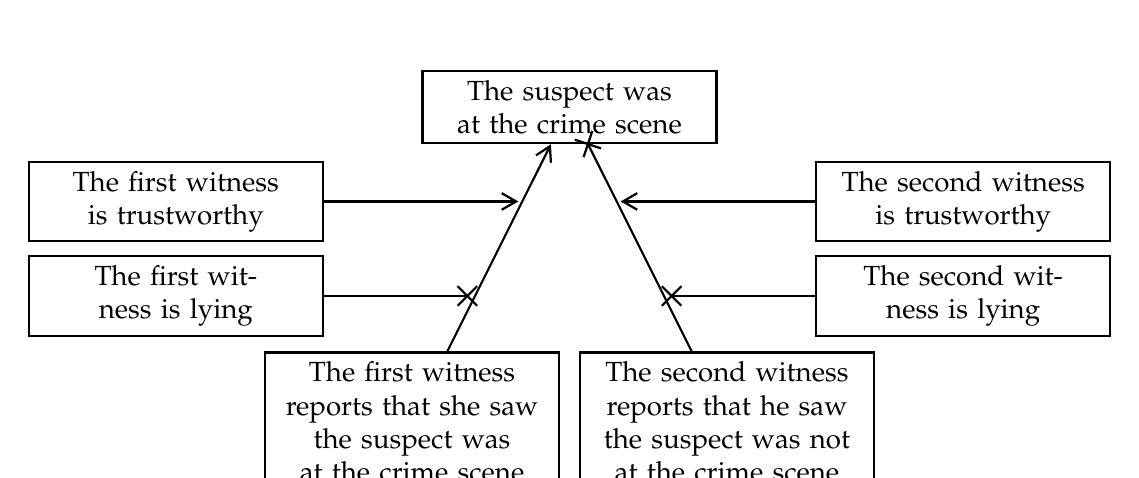
\begin{tikzpicture}[
		scnnode/.append style={text width=3cm},
		arg/.append style={text width=3.5cm},
	]
		\pgftransformxscale{5}
		\pgftransformyscale{2}

		\node[arg]     			(scene) at (0,0) {The suspect was at the crime scene};
		\node[arg] (witn1) at (-0.4,-2) {The first witness reports that she saw the suspect was at the crime scene};
		\node[arg] (witn2) at (0.4,-2) {The second witness reports that he saw the suspect was not at the crime scene};

		\node[arg] 					(trust1) at (-1,-0.6) {The first witness is trustworthy};
		\node[arg] 					(lying1) at (-1,-1.2) {The first witness is lying};
		\node[arg] 					(trust2) at (1,-0.6) {The second witness is trustworthy};
		\node[arg] 					(lying2) at (1,-1.2) {The second witness is lying};

		\draw[arg] 					(witn1) -- (scene);
		\draw[arg]		 			(trust1) -- (-0.13, -0.6);
		\draw[attack] 			(lying1) -- (-0.26, -1.2);

		\draw[attack] 			(witn2) -- (scene);
		\draw[arg]		 			(trust2) -- (0.13, -0.6);
		\draw[attack] 			(lying2) -- (0.26, -1.2);

	\end{tikzpicture}
\end{document}

\caption{Arguments about whether a reason is supporting or attacking\label{fig:nesting}}
\end{figure}

\paragraph{Further readings} Nonmonotonic reasoning~\citep{gabbayEtal1994}. Prima facie reasons, undercutting and rebutting defeaters~\citep{pollock1987, pollock1995}. Warrants and backings~\citep{toulmin1958}. Argument schemes and critical questions~\citep{waltonReedMacagno2008}. 
%Accrual
%Reason-Based Logic

\begin{comment}


\paragraph{Args win when they can defend themselves against attacks (Dung 1995)}

Dung REFERENCE provided an abstract framework to analyze 
systems of arguments. The notion of an argument attacking another argument 
is taken as primitive. We can think of systems of argument as an alliance of arguments, and in particular, 
following Dung's framework, the system $S$ of arguments is a \textit{successful alliance} provided:
%
\begin{quote}
(\textit{conflict-free}) each argument in $S$ is not attacked by any argument in $S$; and 

(\textit{defense}) for any argument (outside $S$) that attacks any argument in $S$, there is an argument inside $S$ that attacks the attacker.
\end{quote}
%
So, a system of arguments forms a successful alliance provided there is no internal conflict and any external attack 
can be counterattacked by arguments within the alliance. The notions of a winning and losing argument can now be defined:
%
\begin{quote}
(\textit{winning})  $A$ \textit{wins} provided $A$ is part of a successful alliance; and 

(\textit{losing} ) $A$ \textit{loses} provided another argument $A'$ attacks $A$ and $A'$ wins. 
\end{quote}
%
These definitions are intuitive. If an argument can defend itself from any attack by appealing to its allies, it wins. If, instead, there is a winning argument that attacks an argument, the latter loses. A problem here, however, is that an argument can be both winning and losing. 
Consider four arguments $A, B$ and $A', B'$ such that $A'$ attacks $A$ and vice versa, and $B$ attacks $B'$ and vice versa. The system $\{A, B\}$ is a successful alliance because there are no internal conflicts and any attack against $A$ or $B$ is counterattacked within the alliance $\{A, B\}$. It follows that arguments $A$ and $B$  both win. At the same time, the system $\{ A', B'\}$ is also 
a successful alliance, so arguments $A'$ and $B'$ win. This means that $A$ and $B$ both lose because each is attacked by a winning argument, and the same holds for $A'$ and $B'$.

%(Intuitively, alliance $\{A, B\}$ and $\{A', B'\}$ are symmetrical in the sense that any argument in one alliance is attacked but an argument in the other alliance. No one appears to be stronger then the other. If, however, we compared $\{A, B, C\}$ and $\{A', B'\}$ and added the condition that $C$ attacks either $A'$ or $B'$ and $\{A, B, C\}$ had no internal conflicts, it would follow that $\{A', B'\}$ is not a successful alliance anymore and thus the only winning arguments would be $A$ and $B$. One easy fix could be to require that successful alliances cannot be symmetrical to other successful alliance. This means for any give set of arguments there is only one successful alliances.)

(As far as evidential reasoning in the law is concerned, something is unsettling about this state of affairs. There is something unnatural about the systems $\{A, B\}$ and $\{A', B'\}$ and the fact that $A$ attack $A'$ and vice versa, and the same holds for $B$ and $B'$.
Suppose an eyewitness asserts she saw the defendant stab the victim and another witness asserts the eyewitness is biased because she has reasons to hate the defendant. The second witness attacks the testimony of the eyewitness. This exemplifies an attack against $A$ by $A'$. There is nothing problematic about that. But now suppose the eyewitness defended herself against the second witness by asserting that the second witness is biased against her because the witness has reasons to hate her. This exemplifies a situation in which $A$ attacks $A'$. There is nothing problematic about that either. But, although the fact that $A$ attacks $A'$ and vice versa are fine as isolated attacks, when they are considered together, they become  problematic. Suppose we engage in a conversation in which I assert conclusion $C$ on the basis of evidence $e$  and you challenge me by challenging $e$ on the basis of other evidence $e'$. Next, I defend myself by challenging your evidence $e'$ and I do so by using my evidence $e$.  You challenge targets $e$ on the basis of $e'$ and I target $e'$ on the basis of $e$. This is a stale mate and a circle of attack and counterattack. Ideally, we would need further evidence, besides $e$ and $e'$, to resolve the controversy. In the court example,  a third witness is needed who can tell us whether the first eyewitness or the second witness is biased. So, an easy fix to the above problem, especially when it comes to evidential reasoning in the law, is to require that stalemate situations or circles of attacks and counterattacks be avoided.)

\paragraph{Args win when they are better/stronger than/preferred over conflicting args}

Dung's framework considers system of arguments and the relations of attack and counterattack among arguments, but does not examine the internal structure of arguments. The notions of attack and counterattack are left unspecified, and the notion of a successful 
attack is also left unspecified. To be sure, all we can say from Dung's framework is that an attack is successful when 
it consists of a winning argument. We are told nothing more about the internal structure of arguments.

 Prakken REFERENCE has provided a unified theory of argumentation which builds on Dung's insights but also examines 
 the internal structure of arguments. As seen earlier, argument can be attacked in three ways. An argument can be attacked by offering another argument with the opposite conclusion (rebutting). An argument can be attacked by offering an argument that weakens the inferential link between premises and conclusion (undercutting). An argument can be attacked by challenging its premises (undermining). The remaining question is, when is an attack successful? 

Let us begin with an example of one argument rebutting another.  A witness asserts that the defendant stabbed the victim, while DNA evidence shows no match between the defendant and the crime traces. The argument based on an witness statements is rebutted by---but also rebuts---the argument based on the DNA match. The attack works in both direction in the sense that bother arguments attack one another regardless of which argument is made first. Is the attack successful? In Dung's framework, the answer is that both arguments win and both arguments lose (provided both arguments are part of a successful alliance). This is hardly satisfying. 

A step forward is a ranking among arguments. A rebutting argument $A'$ is considered a successful attack  on an argument $A$ whenver $A$ is ranked higher than $A'$.  How can arguments be ranked? The ranking will depend on the relative strength we assign to the premises and to the inferential link between premises and conclusion. Consider an abstract example. The first argument consists of premises $A$ and the defeasible inference $A\Rightarrow B$, while the second argument consists of premises $A'$ and the defeasible inference $A'\Rightarrow \neg B$. The conclusion of the first argument is $B$ and the conclusion of the second argument is the negation of $B$. Which argument ranks higher? This will depend on whether we consider $A$ a better premise---for example, more probable---than $A'$. It will also depend on whether we consider $A\Rightarrow B$ a better inference---for example, more likely to preserve the truth---than $A'\Rightarrow \neg B$. Clearly, other things being equal, if $A$ is better than $A'$, the first argument is ranked higher. However, if $A$ is a better premise but $A'\Rightarrow \neg B$ is a better inference, it is not easy to adjudicate the ranking of the two arguments.

Consider now a case in which an argument undercuts another argument. There is nothing peculiar about this case. We can apply the same ideas as in the rebutting case. In order for the attack to be successful, the undercutting argument must be ranked higher than the attacked argument. 
If not, the attack launched by the undercutting argument must fail. 
 
Finally, the third type of attack: undermining. An attack against a premise can consists in a one line statement that the premise is false or can be a more elaborate argument resulting in the denial of the premise. How can we tell which attacks on the premises are successful? At first blush, one mighty say that the mere statement that the premise is false would not do, but this would be too simplistic.  Premises come in different guises and sometimes it might be enough to merely disagree with a premise and some other times a more sustained argument might be necessary. To illustrate, consider three types of premises. REFERENCES TO PRAKKEN AND GORDON

First, premises can be axioms or self evident statements. If the premises are axioms or self evident, they cannot be attacked. An attack against an axiom or a self evident premise will therefore always fail. 

Second, premises can also be assumptions or statements that are taken for granted without explicitly supporting reasons. Assumptions are peculiar in that that they hold until contrary evidence shows they are false. Assumptions are close to what in the law are known as presumptions. Suppose the prosecutor argues that a mail package containing drugs was received by the defendant. The prosecutor has proof that the package was mailed and that it reached the defendant's address. The prosecutor has no explicitly proof that the packed was delivered to the defendant. The prosecutor \textit{assumes} that if the package was sent and received at the defendant's address, it was the defendant who received it. What if the defendant challenges the assumption alleging that he was not at home when the package was delivered? This raises the question of who has the burden of proof. Should the prosecutor give evidence that the assumption is correct or should the defendant give evidence that the assumption is incorrect, and in absence of contrary evidence, should the assumption be taken to be correct? 
If we are in fact dealing with an assumption, it is up to the party who challenges the assumption to show that it is correct. Assumptions are true until contrary evidence is provided. 

Finally, we have ordinary premises. These must be defended with adequate evidence and arguments and cannot be assumed the be true. If the a party attacks an argument by challenging an ordinary premise, the burden of proof is on the party proposing the argument to back up the premise. Ordinary premises, in this sense, are very different from assumptions. In short, axioms or self evident premises cannot be challenged. Assumptions are assumed to hold until contrary evidence is presented. The burden of proof is on the attacking party. Ordinary premises can only be believed on the basis of supporting evidence or arguments. The burden of prof here is on the attacked party. 

An attack against the premises of an argument will succeed or fail depending on the targeted premises. Attacks against self evident premises always fail. Attacks against assumptions are successful only if evidence is introduced that the assumption is indeed false. Attacks against ordinary premises succeeds even though no evidence that the premise is false is introduced and provided that the other party has introduced no evidence for the truth of the premise. If the other party has introduced evidence for the truth of the premise, the premise is the conclusion of an argument, and thus the attack must take form of a rebuttal.



 

 
\end{comment}

\subsection{Scenarios}

The evidential value of a scenario depends on how well it matches up with the evidence. 
This matching up can be understood in three ways: a scenario's consistency 
with the evidence; its power to explain the evidence; 
and its evidential support. Let us consider each in turn.


\paragraph{Scenarios can be plausible and logically consistent.}

Plausibility measures how well a scenario matches up with 
our background assumptions and knowledge of the world. 
%The events that constitute a scenario must be linked by relations of temporal order and causality. 
The scenario should not violate with the laws of nature or common sense. If a scenario asserts that the same individual was in two different locations 
at the same time, or moved from one location to another in too short amount of time, the scenario would lack plausibility.  
The scenario `an alien did it' lacks plausibility because it described soemthign that rarely happens. 
Lack of plausibility can become so pronounced that it amounts to a lack of \textit{logical consistency}, for example, claiming that 
 the defendant had and did \textit{not} have a motive for killing the victim
 
Plausibility has something to do with what we might can \textit{normality}, that is, 
what happens most of the time. A scenario according to which the defendant covered 500 mile of distance by car is more plausible than a scenario in which the
defendant covered the same distance by foot. The former happens more often than the latter. 
Or, suppose the defendant is said to have a lovely relation with 
the victim the day before, while the next day the defendant is depicted as killing the victim out of anger.
The scenario lacks plausibility because it does not happen very often that anger follows a peaceful 
interaction the day before. It is true, however, that criminal cases are often about odd coincidences, 
unexpected and improbable occurrences.  Plausibility only measures the persusiveness of a scenario 
\textit{prior to} considering any more specific evidence about the crime.  An initially plausible scenario can be turn out to be 
not very persuasive in light of more evidence presented about the crime. 

%But the former need not be more plausible than the latter. 
%Consistency with the laws of nature and common sense, whether the parts 
%of the scenario ``hang together'' nicely (cohesiveness and internal consistency) 
%are also indicators of plausibility. 


%The plausibility of a scenario is weakened when the components of the scenario, its
%sub-scenarios, cannot be easily combined together. This could also be understood as 
%a lack of \textit{cohesiveness} among the components of a scenario. So, not only the scenario should explain the evidence, but certain
% components of a scenario should explain others. Typically we expect that events prior in time 
% explain events later in time. 
 
 

%The terminology used here---plausibility, logical consistency, cohesiveness, normality---can be confusing. 
%Still, the main idea is that a scenario can be evaluated against what a reasonable person thinks 
%it would happen given a set of circumstances. 

\paragraph{The more evidence a scenario can explain, the better.}

When a case comprises several items of evidence, 
%the interpretation of the evidence becomes holistic. 
a scenarios's credibility depends on how it can account for the whole mass of evidence.  
 The more items of evidence a scenario can account for, preferably from both the prosecutor and the defense, 
 the better the scenario. This depends on the scenario's consistency with the evidence, 
 explanatory power and evidential support. These criteria were already discussed earlier. 
 The difference now is that consistency, explanatory power and evidential support should 
 be measured relative to the totality of the evidence.  
 
 Suppose two items of evidence must be explained: first, the presence of fingerprints at the crime scene; 
and second the fact that those fingerprints match with the defendant.  Suppose scenario $S_1$ comprises the event that the 
defendant visited the crime scene, while $S_2$ compromises the event that some other individual visited the crime scene. Both scenarios 
explain the presence of fingerprint traces, but only $S_1$ can explain the fact that the traces match with the defendant. Now, a third scenario $S_3$ in which another individual visited the crime and  implanted fingerprints that match the defendant can explain both items of evidence. As far as explanatory power goes, scenarios $S_1$ and $S_3$ are equal, although further evidence may distinguish them. For example, if a witness testified that she saw the defendant walk towards the location of the crime when the crime was committed, scenario $S_3$ could 
not easily explain the testimony, while $S_1$ could. So, absent other evidence, scenario $S_1$ explains more evidence than the other competing scenarios. 
 

\paragraph{Scenarios must be consistent with the evidence.}

We can evaluate a scenario by checking whether it is consistent with the evidence presented in a case.
If a witness testifies that the defendant was at home with his girlfriend 
at 6 PM, while according to the scenario proposed by the prosecutor, 
the defendant was at the crime scene at 6 PM, the 
two are inconsistent. More precisely, insofar as the evidence 
is taken at face value---that is, the witness is taken to be truthful---the scenario 
is inconsistent with the evidence. A \textit{prima facie} inconsistency 
between the evidence and a proposed scenario need not be damning for the scenario's credibility, 
but at least, it calls for further investigating.  It might, of course, turn out that the witness was untruthful or simply confused about 
the timing.  If so, the evidence will be discarded, not the scenario. But, there are cases in which the evidence 
cannot be easily discarded. Suppose a video recording shows the defendant went into a bank 
and committed a robbery, and instead, the scenario proposed by the defense denies precisely that. The defense 
will be hard pressed to justify the proposed scenario given the inconsistency 
with the evidence. 




\paragraph{Further readings}

Explanation in the deductive nomological model \citep{hempelOppenhaim1948}. 
Explanation and causality \citep{salmon1984}. 
Abduction and inference to the best explanation \citep{lipton1991}.
More the philosophical literature on 
scientific explanation \citep{woodward2014}. 
Two directions of fit \citep{wells1992}.


\section{Coherently interpreting the evidence}
\label{sec:cohint}

The dossiers of criminal cases can be large, and the coherent interpretation of the evidence in such a dossier can 
be daunting, whichever normative framework is used. For each framework, we discuss how the coherent 
interpretation of the evidence can be addressed.

\subsection{Scenarios}

%In the previous section, we evaluated scenarios by how well they matched up with the evidence, in terms of consistency, explanatory power and evidential support.
%These were atomistic criteria. 

Scenarios can provide coherent interpretations that make sense of the evidence.
  
\paragraph{Scenarios are clusters of events, ordered in time and connected by causal relations.} Consider again a murder example with two suspects: the victim's former partner, who killed the victim after a fight ($S_1$), and a robber who killed the victim when caught during a robbery ($S_2$). Scenario $S_1$ can be made explicit as a sequence of four hypothetical consecutive events (Figure~\ref{fig:scens}). First, the victim and his former partner have a relation ($H_1$); then they break up ($H_2$); subsequently, there is a fight ($H_3$); and finally, the victim is killed by his former partner ($H_4$). Scenario $S_2$ can be analyzed as consisting of three events. First, the robber enters the victim's house ($H_5$); then the victim accidentally encounters the robber ($H_6$); and finally, the robber kills the victim ($H_7$). Some of the events in these chronologically ordered scenarios are causally connected. For instance, in the first scenario, the killing is caused by the break up and the fight; and in the second scenario by the accidental encounter.

\begin{figure}[bt]
\centering
\documentclass[border=5mm,tikz]{standalone} 

\usepackage{amsmath}
% !TEX root=img/arguments_and_attack.tex

% \usetikzlibrary{external} 
% \tikzexternalize[prefix=tikz/] 

\usetikzlibrary{calc}
\usetikzlibrary{arrows}
\usetikzlibrary{arrows.meta}
\usetikzlibrary{decorations.markings}
% \usetikzlibrary{intersections}
\usetikzlibrary{fit}
\usetikzlibrary{shapes}
% \usetikzlibrary{trees}


\tikzset{
	every path/.style={thick},
	align=center,
	observed/.style={
		fill=black!20,
	},
	bn/.style={
		draw,
		ellipse,
		-{Triangle[angle=60:6pt 0]}
	},
	scn/.style={
		draw,
		rectangle,
		% signal,
		% signal from=west,
		% signal pointer angle=120,
		-{Triangle[angle=60:6pt 0]},
	},
	possibly/.style={dashed},
	arg/.style={
		draw,
		rectangle,
		-{Straight Barb[angle=60:6pt 0]}
	},
	attack/.style={
		-{Rays[width=10pt,length=10pt,sep=-3.9pt]}
	},
	pref/.style={
		draw,
		rectangle,
		-{Straight Barb[angle=60:6pt 0]}
	},
	subscn/.style={
		double,
		-{Triangle[angle=60:6pt 0]},
	},
	specific/.style={
		double,
		-{Stealth[angle=60:6pt 0]}
	},
}



\begin{document}
	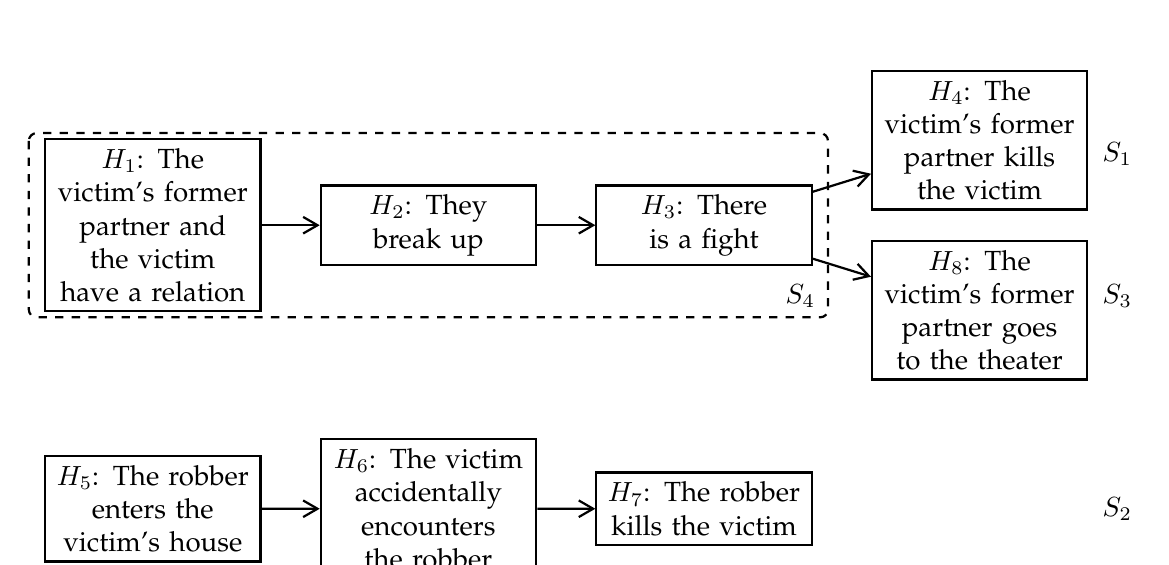
\begin{tikzpicture}[
		scn/.append style={text width=2.5cm},
		arg/.append style={text width=3cm},
	]
		\pgftransformxscale{3.5}
		\pgftransformyscale{1.8}
		
		\node[scn] (H1) at (1,0) {$H_1$: The victim's former partner and the victim have a relation};
		\node[scn] (H2) at (2,0) {$H_2$: They break up};
		\node[scn] (H3) at (3,0) {$H_3$: There is a fight};

		\node[scn] (H4) at (4,0.6) {$H_4$: The victim's former partner kills the victim};

		\node at (4.5,0.5) {$S_1$};

		\node[scn] (H8) at (4,-0.6) {$H_8$: The victim's former partner goes to the theater};

		\node at (4.5,-0.5) {$S_3$};

		\node[scn] (H5) at (1,-2) {$H_5$: The robber enters the victim's house};
		\node[scn] (H6) at (2,-2) {$H_6$: The victim accidentally encounters the robber};
		\node[scn] (H7) at (3,-2) {$H_7$: The robber kills the victim};

		\node at (4.5,-2) {$S_2$};

		\draw[thick,dashed,rounded corners=1mm] (0.55,0.65) rectangle (3.45,-0.65);
		\node at (3.35,-0.5) {$S_4$};

		\draw[arg] (H1) -- (H2);
		\draw[arg] (H2) -- (H3);
		\draw[arg] (H3) -- (H4);
		\draw[arg] (H3) -- (H8);
		\draw[arg] (H5) -- (H6);
		\draw[arg] (H6) -- (H7);


	\end{tikzpicture}
\end{document}

\caption{Alternative scenarios and their structure\label{fig:scens}}
\end{figure}



\paragraph{Scenarios can be more or less complete.}

Another criterion to evaluate scenarios is their \textit{completeness}. Since scenarios are discursive arrangement of events, ordered according to 
temporal and causal relations, they may contain gaps in time, space and causality. A scenario may not describe the defendant's whereabouts between 4 and 6 PM, 
while it describes, rather precisely, what the defendant did at 7 PM, immediately before the killing took place. The temporal gap between 4 and 6 PM 
makes it less complete than a scenario which describes the defendant's whereabouts between 4 and 7 PM without gaps. 
Yet, this might not be the notion of completeness that is important here.  

%Completeness depends on factors such as relevance, causal structure and expectations. 
In a murder case, the identity of the perpetrator, the motive, the 
modus operandi of the crime and the weapon are relevant items which a scenario should specify. 
The lack of any of these from a proposed scenario would make it incomplete. 
The law itself sometimes requires that specific items be proven, 
for example, in criminal cases both the \textit{mens rea} and \textit{actus reus} 
must be proven.   Still, the law does not say whether the defendant's whereabouts the day before or a month before 
the murder are relevant. They could be relevant to establish motive or they might not. 
This depends on the circumstances of the case. So, how is completeness a criterion to evaluate 
a scenario? Some suggest that scenarios must follow certain patterns, 
schematic structure or scripts. For example, in most violent crimes, we can identify an initial 
moment of conflict, which triggers a specific psychological reaction that gives rise to the formation of an 
intention, which, in turn, later results in the violent act. On this account, a scenario is 
complete whenever it has all of its parts, at least given an appropriate scenario script.
The notion of completeness, then, overlaps with 
that of plausibility and cohesiveness of a scenario.

All in all, evaluating a scenario required different levels of analysis: consistency with the evidence; 
explanatory power (predictive power and causal fit); evidential support; plausibility 
(and also, cohesiveness, internal consistency and normality); completeness.




\paragraph{Scenarios considered may or may not solve a case, and show which evidence is legally relevant.} A criminal case is only solved when the legally relevant circumstances can be proven. For instance, in murder cases, it should be proven who killed the victim and why. Of the scenarios considered, the former partner murder scenario $S_1$ and the robbery murder scenario $S_2$ explain how and why the murder happened, but the alibi scenario $S_3$ does not. In a crime investigation, it can be hard to find evidence that proves a sufficiently detailed scenario about what has happened. For instance, in the example, it is initially clear that a murder had happened, but not by who. Because of the break up, a scenario that answers the why-question is considered: the former partner murder scenario $S_1$. That scenario is initially corroborated by the DNA match $E_1$, but then breaks down by the use of the bank card $E_2$ that proves the alibi scenario $S_3$. Only when the robber is caught and confesses having killed the victim (evidence $E_3$)---possibly much later, it becomes clear what has happened. The body found $E_0$ and the confession $E_3$ are relevant for answering the legally relevant questions who killed the victim and why. The other evidence considered, the DNA match $E_1$ and the use of the bank card $E_2$, have played a relevant role in the investigation, but do not support or contradict robbery murder scenario $S_2$. 

			%E0			E1			E2			E3
%S1		expl		expl		ind			ind
%S2 		expl		ind			ind			expl
%
%S3		ind			expl		expl		ind
%
%S4		ind			expl		ind			ind
%S2+S3	expl		expl		expl		expl



\paragraph{Further readings}

Explanation and unification 
in philosophy of science \citep{friedman1974}. 
Coherence in epistemology \citep{bonjour1985}.
The crossword puzzle analogy for coherently 
evaluating a mass of evidence \citep{haack2008}.
Explanatory coherence \citep{thagard2001}.
The story model \citep{penningtonHastie1993StoryModel}. 
Scenarios as scripts \citep{wagenaarEtal1993}.
Scenarios in legal cases \citep{griffin2013}. 
Worries about scenarios in law \citep{velleman2003}.






\subsection{Arguments}
\label{sec:coh-arg}

An analysis of a case in terms of arguments can become very complex. This was already noted by Wigmore, when he developed his charting method for analyzing the evidence in a criminal case~\citep{wigmore1913,wigmore1931}. Figure~\ref{fig:wigmore} provides an example of a Wigmore diagram (\citeyear{wigmore1931}). Here Wigmore has analyzed a murder case (Commonwealth v. Umilian, 1901). Jedrusik, the victim, was the author of a letter in which he falsely advised a priest that Umilian had a wife and children (back in the country from which they emigrated), conflicting with Umilian’s intention to marry. In the chart, Z stands for the charge that Umilian killed Jedrusik. The node at 8 represents a revengeful murderous emotion toward Jedrusik. At 18, it is represented that the marriage is in the end performed, reducing his feelings of revenge. This claim is supported by the (unspecified) evidence at 18.1. The diagram contains some two dozen nodes. Diagrams for more complex cases can contain many more nodes.

\begin{figure}[bt]
	\centering
		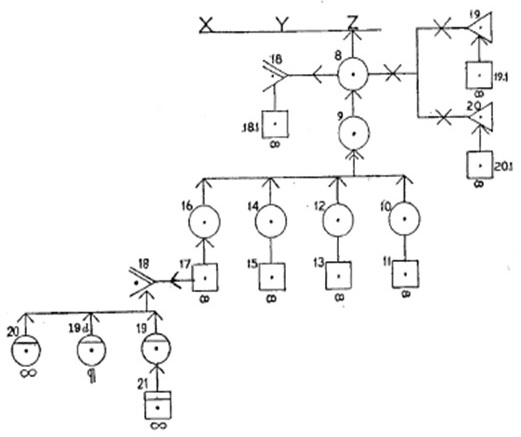
\includegraphics[scale=0.7]{img/wigmore.jpg}
\caption{A Wigmore chart\label{fig:wigmore}}
\end{figure}

\paragraph{The evaluation of an argument can depend on its subarguments.}Given an argumentative analysis of the case, one would like to know which conclusions follow, and which don't. 
%We already discussed how arguments consisting of conflicts of reasons can be evaluated in this sense, when we discussed the role of exceptions, preferences and weighing (Section~\ref{sec:valueArgs}). 
The structure of a complex of arguments influences the evaluation of the arguments, and in particular, the subarguments of a larger argument determine the evaluation of the whole. 
For example, consider the argument in Figure~\ref{fig:arg2} (page~\pageref{fig:arg2}). There the witness testimony supported the intermediate conclusion that the suspect was at the crime scene, which in turn supported the conclusion that the suspect committed the crime. So there is an argument consisting of two steps. In the example, the first of these steps is attacked by a counterargument involving the lying of the witness. As a result of this attack, the argument to the intermediate conclusion that the suspect was at the crime scene breaks down and its conclusion does not follow. As a result, also the larger two-step argument no longer supports its conclusion, which hence does not follow. Since the one-step subargument does not successfully support the intermediate conclusion, also the whole two-step argument for the final conclusion does not successfully support its conclusion.

\paragraph{The evaluation of an argument can depend on chains of attacks.} When an argument is successfully attacked, it no longer successfully supports its conclusion. But attack can be chained, since the attack itself can be countered by a further attack. When an attack is successfully attacked, the original argument can be reinstated, in the sense that it again successfully supports its conclusion. Figure~\ref{fig:reinstatement} shows an example. A first witness, Witness $A$, reports that the suspect was at the crime scene. Given only this information, there is good reason to assume that the suspect was at the crime scene. However, there is a second witness, Witness $B$, who reports that Witness $A$ is lying. Given these two reasons, based on the witness reports by $A$ and $B$, it is no longer successfully supported that the suspect was at the crime scene. If now there is a third witness, Witness C, who reports that Witness B is lying, the attack is countered. Witness B is no longer believed, so there is no reason to conclude that Witness A is lying. As a result, A's report can again support its conclusion that the suspect was at the crime scene. The original argument based on A's report is reinstated. 

\paragraph{Conflicts between reasons can be addressed by exceptions, preferences and weighing [NEEDS FIXING].} The counterarguments to a reason that result from asking critical questions give rise to conflicts between reasons. Sometimes conflicts of reasons can be resolved in the sense that it can be determined which conclusions follow from the conflicting reasons. We distinguish three kinds of conflicts. 

In the first kind of conflicts between reasons, there is a reason attacked by an exclusionary reason, i.e., an attack of the undercutting kind that goes against the connection between the reason and its conclusion (cf. Section~\ref{sec:confArg}). This situation is shown at the top of Figure~\ref{fig:conflicts}: There is a witness reporting that the suspect was at the crime scene, but there is evidence that the witness is lying. 
%BV Done [ISN'T IT BETTER TO SAY THAT THERE IS EVIDENCE SUGGESTING THAT THE WITNESS IS LYING? ] 
In that case, the conclusion that the suspect was at the crime scene does not follow, since there is no supporting reason for it. The reason (the witness report itself) and the exception (the lying of the witness) both hold as they are assumptions. %MDB [DID YOU INTRODUCE THE IEDA OF ASSUMPTION ALREADY? IS IT NECESSARY?]
In this situation of a reason with an undercutting attack by an exclusionary reason, the conflict of reasons is resolved by the exception expressed in the exclusionary reason. 
%MDB [NOT SURE I UNDERSTAND HOW THE CONFLICT IS RESOLVED HERE. THE UNDERCUTTING REASON WINS. OK. BUT HOW IS THIS A RESOLUTION OF THE CONFLICT?]

\begin{figure}[bt]
\centering
\documentclass[border=5mm,tikz]{standalone} 

\usepackage{amsmath}
% !TEX root=img/arguments_and_attack.tex

% \usetikzlibrary{external} 
% \tikzexternalize[prefix=tikz/] 

\usetikzlibrary{calc}
\usetikzlibrary{arrows}
\usetikzlibrary{arrows.meta}
\usetikzlibrary{decorations.markings}
% \usetikzlibrary{intersections}
\usetikzlibrary{fit}
\usetikzlibrary{shapes}
% \usetikzlibrary{trees}


\tikzset{
	every path/.style={thick},
	align=center,
	observed/.style={
		fill=black!20,
	},
	bn/.style={
		draw,
		ellipse,
		-{Triangle[angle=60:6pt 0]}
	},
	scn/.style={
		draw,
		rectangle,
		% signal,
		% signal from=west,
		% signal pointer angle=120,
		-{Triangle[angle=60:6pt 0]},
	},
	possibly/.style={dashed},
	arg/.style={
		draw,
		rectangle,
		-{Straight Barb[angle=60:6pt 0]}
	},
	attack/.style={
		-{Rays[width=10pt,length=10pt,sep=-3.9pt]}
	},
	pref/.style={
		draw,
		rectangle,
		-{Straight Barb[angle=60:6pt 0]}
	},
	subscn/.style={
		double,
		-{Triangle[angle=60:6pt 0]},
	},
	specific/.style={
		double,
		-{Stealth[angle=60:6pt 0]}
	},
}



\begin{document}
	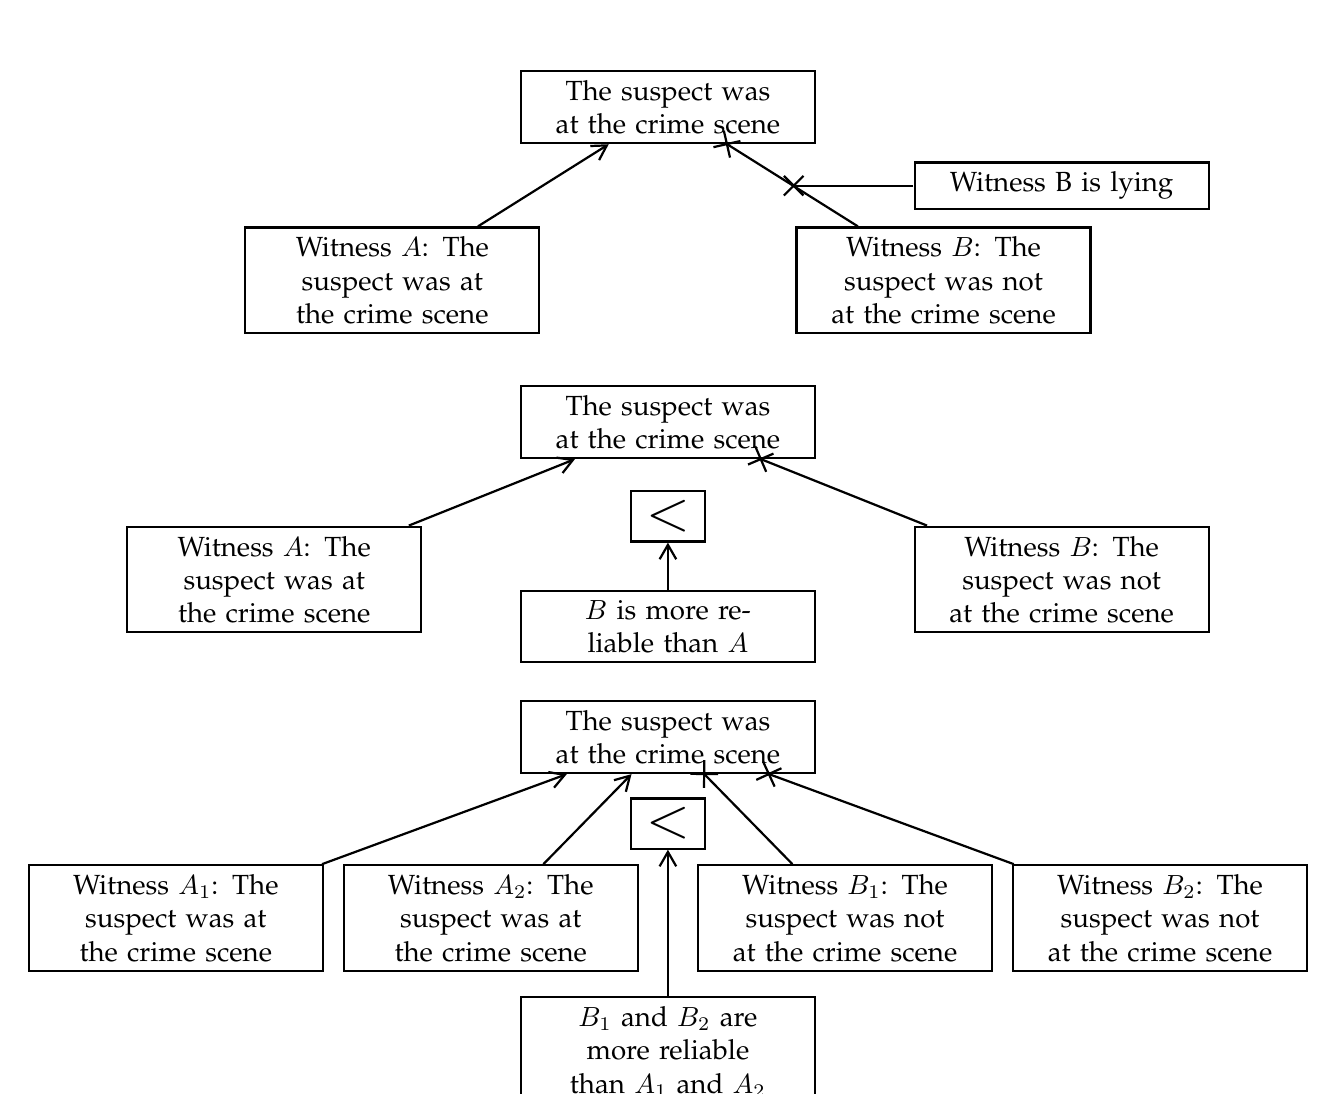
\begin{tikzpicture}[
		scnnode/.append style={text width=3cm},
		arg/.append style={text width=3.5cm},
		pref/.append style={text width=0.7cm},
	]
		\pgftransformxscale{5}
		\pgftransformyscale{2}

		\node[arg]     			(scene) at (0,0) {The suspect was at the crime scene};
		\node[arg] (witn) at (-0.7,-1.1) {Witness $A$: The suspect was at the crime scene};
		\node[arg] (witn2) at (0.7,-1.1) {Witness $B$: The suspect was not at the crime scene};

%		\node[arg] (witn) at (0,-1.1) {Witness: The suspect was at the crime scene};

		\node[arg] 					(lying) at (1,-0.5) {Witness B is lying};

		\draw[arg] 					(witn) -- (scene);
		\draw[attack] 					(witn2) -- (scene);
		\draw[attack] 			(lying) -- (0.32, -0.5);

%*********

		\node[arg]     			(scene) at (0,-2) {The suspect was at the crime scene};
		\node[arg] (witn) at (-1,-3) {Witness $A$: The suspect was at the crime scene};
		\node[arg] (witn2) at (1,-3) {Witness $B$: The suspect was not at the crime scene};

		\draw[arg] 					(witn) -- (scene);
		\draw[attack] 			(witn2) -- (scene);

		\node[pref] 				(pref) at (0,-2.6) 	{\huge $<$};
		\node[arg] 					(rel) at (0,-3.3) 		{$B$ is more reliable than $A$};

		\draw[arg] 					(rel) -- (pref);

%*********

		\node[arg]     			(scene) at (0,-4) {The suspect was at the crime scene};
		\node[arg] (witn) at (-1.25,-5.15) {Witness $A_1$: The suspect was at the crime scene};
		\node[arg] (witn2) at (-0.45,-5.15) {Witness $A_2$: The suspect was at the crime scene};
		\node[arg] (witn3) at (0.45,-5.15) {Witness $B_1$: The suspect was not at the crime scene};
		\node[arg] (witn4) at (1.25,-5.15) {Witness $B_2$: The suspect was not at the crime scene};

		\draw[arg] 					(witn) -- (scene);
		\draw[arg] 					(witn2) -- (scene);
		\draw[attack] 			(witn3) -- (scene);
		\draw[attack] 			(witn4) -- (scene);

		\node[pref] 				(pref2) at (0,-4.55) 	{\huge $<$};
		\node[arg] 					(outweigh) at (0,-6) 		{$B_1$ and $B_2$ are more reliable than $A_1$ and $A_2$};

		\draw[arg] 					(outweigh) -- (pref2);



	\end{tikzpicture}
\end{document}

\caption{Three kinds of conflicts and their resolution\label{fig:conflicts}}
\end{figure}

In the second kind of conflicts between reasons, there is one reason for a conclusion and another against the conclusion. For instance, there are two witnesses with opposite reports about whether the suspect was at the crime scene or not (see the middle of Figure~\ref{fig:conflicts}). This is an example of a rebutting attack (Section~\ref{sec:confArg}). The conflict of reasons is unresolved given only the reasons. Further information about the reasons is required to resolve the conflict. The resolution of such a conflict of reasons can be thought of as the preference of one over the other. A reason can be preferred over another, for instance when it is stronger. In the example, the preference (in the figure indicated by the $<$-sign) is argued for by the claim that one of the witnesses is more reliable than the other. In this case, the conclusion follows that the suspect was not at the crime scene, given this conflict of reasons and its resolution. 

The third kind of conflicts between reasons discussed here involves more than two reasons. For instance, there are more than two witnesses, with conflicting reports (Figure~\ref{fig:conflicts}, bottom). In the figure, both sides are supported by two witness reports. Resolving such a conflict can be thought of as a weighing of the reasons, generalizing the preference between two conflicting reasons. Again, it is concluded that the suspect was not at the crime scene, given this resolution of this conflict of reasons.

%MDB [I THOUGHT THE THREE TYPES OF CONFLICTS MIRRORED THE DISTINCTIONS BETWEEN UNDERCUTTING, REBUTTING AND UNDERMINING, BUT THE THIRD CONFLICT YOU DISCUSS HERE IS DIFFERENT FROM UNDERMINING. IS THIS INTENDED?]




\begin{figure}[bt]
\centering
\documentclass[border=5mm,tikz]{standalone} 

\usepackage{amsmath}
% !TEX root=img/arguments_and_attack.tex

% \usetikzlibrary{external} 
% \tikzexternalize[prefix=tikz/] 

\usetikzlibrary{calc}
\usetikzlibrary{arrows}
\usetikzlibrary{arrows.meta}
\usetikzlibrary{decorations.markings}
% \usetikzlibrary{intersections}
\usetikzlibrary{fit}
\usetikzlibrary{shapes}
% \usetikzlibrary{trees}


\tikzset{
	every path/.style={thick},
	align=center,
	observed/.style={
		fill=black!20,
	},
	bn/.style={
		draw,
		ellipse,
		-{Triangle[angle=60:6pt 0]}
	},
	scn/.style={
		draw,
		rectangle,
		% signal,
		% signal from=west,
		% signal pointer angle=120,
		-{Triangle[angle=60:6pt 0]},
	},
	possibly/.style={dashed},
	arg/.style={
		draw,
		rectangle,
		-{Straight Barb[angle=60:6pt 0]}
	},
	attack/.style={
		-{Rays[width=10pt,length=10pt,sep=-3.9pt]}
	},
	pref/.style={
		draw,
		rectangle,
		-{Straight Barb[angle=60:6pt 0]}
	},
	subscn/.style={
		double,
		-{Triangle[angle=60:6pt 0]},
	},
	specific/.style={
		double,
		-{Stealth[angle=60:6pt 0]}
	},
}



\begin{document}
	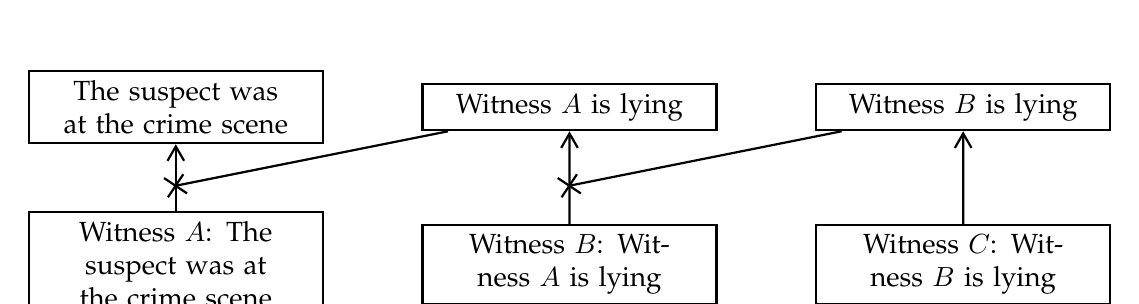
\begin{tikzpicture}[
		scnnode/.append style={text width=3cm},
		arg/.append style={text width=3.5cm},
	]
		\pgftransformxscale{5}
		\pgftransformyscale{2}

		\node[arg]     			(scene) at (0,-1) {The suspect was at the crime scene};
		\node[arg] (witn) at (0,-2) {Witness $A$: The suspect was at the crime scene};

		\draw[arg] 					(witn) -- (scene);

		\node[arg] 					(lying) at (1,-1) {Witness $A$ is lying};
		\node[arg] (witnB) at (1,-2) {Witness $B$: Witness $A$ is lying};

		\draw[attack] 			(lying) -- (0, -1.5);
		\draw[arg] 					(witnB) -- (lying);

		\node[arg] 					(lying2) at (2,-1) {Witness $B$ is lying};
		\node[arg] (witnC) at (2,-2) {Witness $C$: Witness $B$ is lying};

		\draw[attack] 			(lying2) -- (1, -1.5);
		\draw[arg] 					(witnC) -- (lying2);

	\end{tikzpicture}
\end{document}

\caption{Reinstatement\label{fig:reinstatement}}
\end{figure}


\paragraph{Further readings}
Argument structure and their evaluation~\citep{pollock1995}. Formalizing argumentation~\citep{prakkenVreeswijk2002}. Evaluating argument attack~\citep{dung1995}. 
Formal argumentation models~\citep{simariLoui1992, vreeswijk1997, prakken2010, verheij2003deflog, gordonEtal2007}. 

%\paragraph{Inference to the best explanation (Allen/Pardo?)}

%\paragraph{WORRY: Confused about this one; why is it under coherence?) [Answer BV: Otherwise nothing remains here. ]}



\subsection{Probability}

The probability calculus provides formal rules for the coherent interpretation of the evidence.

%\paragraph{The likelihood ratio formula shows how new evidence changes the odds of a hypothesis.} 

\paragraph{The likelihood ratio formula shows how to find the posterior odds given the evidence.} 
The odds of a hypothesis $H$ are defined as the ratio $P(H)/P(\neg H)$ of the probability of the hypothesis and the probability of its negation. Given evidence $E$, the odds $P(H)/P(\neg H)$ 
of the hypothesis unconditioned on the evidence are called the \emph{prior odds} of the hypothesis, and the odds $P(H | E)/P(\neg H | E)$ of the hypothesis 
conditioned on the evidence the \emph{posterior odds}.\endnote{The language of 'priors' and 'posteriors' is standard and suggests 
an temporal ordering.  However, these probabilities are all assigned at the same time; they are not temporally ordered. Contrast this with 
\textit{Bayesian updating} which is the controversial epistemological thesis 
that the probability of $H$ \textit{after} considering evidence $E$ at time $t_2$ must be equivalent to the condition probability 
$P(H|E)$ earlier at time $t_1$.} It follows from Bayes' theorem (Section~\ref{sec:normfram:prob}) that the posterior odds can 
be found by multiplying the prior odds with the likelihood ratio: 

	\[ \frac{P(H|E)}{P(\neg H | E)} = \frac{P(E | H)}{P(E| \neg H)}\cdot \frac{P(H)}{P(\neg H)}.\endnote{To derive the likelihood ratio, 
	one first applies Bayes' theorem to both $H$ and $\neg H$. We get $\Pr(H|E) = \Pr(E|H)\cdot\Pr(H)/\Pr(E)$ and $\Pr(\neg H|E) = \Pr(E|\neg H)\cdot\Pr(\neg H)/\Pr(E)$. Using these, we find:

\begin{equation*}
\frac{\Pr(H|E)}{\Pr(\neg H|E)}
=
\frac{\Pr(E|H)\cdot\Pr(H)/\Pr(E)}
{\Pr(E|\neg H)\cdot\Pr(\neg H)/\Pr(E)}
=
\frac{\Pr(E|H)\cdot\Pr(H)}
{\Pr(E|\neg H)\cdot\Pr(\neg H)},
\end{equation*}

\noindent proving the likelihood ratio formula.}\]

\noindent 
This formula shows that an estimate of the (incremental) evidential value of the evidence for a hypothesis, expressed by the likelihood ratio $\frac{P(E | H)}{P(E| \neg H)}$, 
does not by itself give an estimate of the posterior odds of a hypothesis. One needs an estimate of the prior odds too. 
%As such, the likelihood ratio is a constraint that must be obeyed in a coherent interpretation of the evidence concerning a hypothesis.

To arrive at the \textit{posterior probability} $P(H|E)$ of a hypothesis conditional 
on the evidence, from the posterior odds $\frac{P(E|H)}{P(E|\neg H)}$
of the hypothesis given the evidence, the following formula applies:
%
\[P(H|E) = \frac{\frac{P(E|H)}{P(E|\neg H)}}{1+ \frac{P(E|H)}{P(E|\neg H)}}. \]
%

Consider an example. The incremental evidential value of a DNA match, relative to the hypothesis 
that the defendant is guilty, is given by the the likelihood ratio $\frac{P(M |G)}{P( M | \neg G)}$. 
Suppose this ratio is assigned a numerical value,  as follows:
%
\[\frac{P(M |G)}{P( M | \neg G)}=\frac{1}{\frac{1}{2,000,000}}=2, 000,000.\]
% 
Suppose, also, that the prior odds are as follows:
%
\[\frac{P(G)}{P(\neg G)}=\frac{\frac{1}{\text{200,000}}}{\frac{199,999}{200,000}}\approx \frac{1}{200,000}.\]
% 
The posterior odds of the hypothesis given the match $\frac{P(G|M)}{P(\neg G|M)}$ are therefore as follows:
%
\[\frac{P(G|M)}{P(\neg G|M)}= \frac{P(M |G)}{P( M | \neg G)}\cdot \frac{P(G)}{P(\neg G)} \approx 2,000,000 \cdot \frac{1}{200,000}=\frac{20}{1}.\]
% 
So the poster probability of the hypothesis is as follows:
%
\[P(G|M)= \frac{\frac{P(M|G)}{P(M|\neg G)}}{1+ \frac{P(M|S)}{P(M|\neg G)}} \approx \frac{20}{1+20}\approx 0.95.\]
%
 


\paragraph{A generalization of the formula shows how to handle more pieces of evidence.} 
So far we have considered only one piece of evidence. 
%The likelihood ratio formula to more than one piece of evidence, the posterior odds are found by the repeated multiplication of the likelihood ratios of the individual pieces of evidence. 
For two pieces of evidence $E_1$ and $E_2$, the formula can be generalized 
by multiplying the likelihood ratios of the individual pieces of evidence, as follows:
	\[ \frac{P(H|E_1 \land E_2)}{P(\neg H | E_1 \land E_2)} = 
	\frac{P(E_2 | H)}{P(E_2| \neg H)}
	\cdot 
	\frac{P(E_1 | H)}{P(E_1| \neg H)}
	\cdot 
	\frac{P(H)}{P(\neg H)}.\]
%\noindent Appealing as it is, this naive generalization is false in general and does not hold in the probability calculus. 
This simple generalization holds provided that the two pieces of evidence are 
independent conditional on the hypothesis, that is, $P(E_2| H)=P(E_2| H \wedge E_1)$. 
(More on this below.) 

To illustrate, consider now two pieces of evidence: a DNA match and a witness testimony.
The DNA match, call it $M$, holds between the crime traces and the defendant, and 
the witness, call it $W$, in her testimony asserts that the defendant was 
seen at the crime scene.  
Both pieces of evidence, intuitively, support the hypothesis $G$ that the defendant 
is guilty. To assign an explicit numerical value, assume
 the DNA match has a likelihood ratio $\frac{P(M | G)}{P( M | \neg S)}$ of 2 million, 
and the witness testimony a likelihood ratio $\frac{P(W | G)}{P( W | \neg G)}$ of 1,000. 
These numbers are purely illustrative, but are needed to perform the probabilistic calculations.\endnote{Of course, there remains the 
question of how the numbers can obtained and whether the numbers 
needed to carry out the calculations are always available in the first place. 
This is a topic of debate.}  Finally, assume the two pieces are independent conditional on the hypothesis $G$, that is, 
$P(W|G)=P(W| G\wedge M)$. 

The combined (incremental) evidential value of the two pieces of evidence is given by multiplying the two likelihood 
ratios, that is, $2,000,000\times 1,000=2,000,000,000$, which is a higher value 
than the two pieces considered independently. 
If the prior odds $\frac{P(G)}{P(\neg G)}$ are roughly $\frac{1}{200,000}$
as before, the posterior odds are therefore as follows:
%
\[\frac{P(G|M|\wedge W)}{P(\neg S|M\wedge W)}= \frac{P(M |G)}{P( M | \neg S)}\cdot  \frac{P(W |G)}{P( W | \neg G)}\cdot \frac{P(G)}{P(\neg G)} \approx 2,000,000 \cdot  1,000 \cdot \frac{1}{200,000}= \frac{20,000}{1}.\]
% 
So the poster probability of the hypothesis given the two pieces of evidence is as follows:
%
\[P(G|M\wedge W) \approx \frac{20,000}{1+20,000}\approx 0.99.\]
%
Compare this probability with $P(G|M)$, which 
was 0.95, a lower value. The probability calculus can offer a numerical 
representation of the intuitive fact that two pieces of evidence, taken together, 
have a higher (overall) evidential value than one piece of evidence alone. 

 If the two pieces of evidence are no independent, 
the likelihood ratio formula for two pieces of evidence 
takes the following, more general 
form:

	\[ \frac{P(H|E_1 \land E_2)}{P(\neg H | E_1 \land E_2)} = 
	\frac{P(E_2 | H \land E_1)}{P(E_2| \neg H \land E_1)}
	\cdot 
	\frac{P(E_1 | H)}{P(E_1| \neg H)}
	\cdot 
	\frac{P(H)}{P(\neg H)}.\]

\noindent It is easy to see the first, simple generalization follows from the second, assuming 
independence between the two pieces of evidence conditional on the hypothesis of interest. 
The first generalization does not always hold because 
the evidential value of a piece of evidence, as measured by the likelihood ratio, 
can change in the face of other evidence. The problem with the second formula, however, is that it 
is much more difficult to apply.





%Note how the factor $P(E_2 | H)/P(E_2| \neg H)$ in the naive, incorrect generalization has been replaced by the factor $P(E_2 | H \land E_1)/P(E_2| \neg H \land E_1)$ in the correct generalization.

 %Formally, $P(E_2 | H)/P(E_2| \neg H)$ is in general different from $P(E_2 | H \land E_1)/P(E_2| \neg H \land E_1)$. Evidence can for instance be mutually strengthening. 

% For instance H  E1 E2
%              -  -  -   81
%              -  -  +    9
%              -  +  -    9
%              +  +  +    1
%              Total    100
% E1 and E2 are independent, but mutually strengthening as evidence for H. In fact, LR(E2, H) = 11, LR(E2, H |E1) = infinite. 




\paragraph{The formula can be generalized to calculate the probability of a composite hypothesis, although one should we wary 
of the independence assumptions used.} 
Consider now two hypotheses, $H_1$ and $H_2$, each supported by an item of 
evidence, $E_1$ and $E_2$, respectively.  Can the likelihood ratio formula be generalized to cases with 
two items of evidence and two hypotheses combined? Assuming that the two pieces of evidence are independent, conditional on the hypotheses, 
and the two hypotheses are also independent, 
it is enough to simply multiply the two likelihood ratios, as follows:
%
\[ \frac{P(H_1\wedge H_2|E_1 \land E_2)}{P(\neg H | E_1 \land E_2)} = 
	\frac{P(E_2 | H_2)}{P(E_2| \neg H_2)}
	\cdot 
	\frac{P(E_1 | H_1)}{P(E_1| \neg H_1)}
	\cdot 
	\frac{P(H_1)}{P(\neg H_1)}\cdot \frac{P(H_2)}{P(\neg H_2)}.\endnote{}\]
%

To illustrate, suppose a DNA match links the defendant to the crime scene, while an email written by the defendant indicates 
he had a plan to kill the victim. Each of these item of evidence support a different hypothesis, abbreviated
 \textit{contact} and \textit{plan}.
 %
\begin{comment}
Observe that:
 %
\[ \frac{P(\textit{contact}\wedge \textit{plan} | \textit{match} \wedge \textit{email})}{P(\neg (\textit{contact} \wedge \textit{plan}) |  \textit{match} \wedge \textit{email})} 
=
\frac{P(\textit{match} \wedge \textit{email} | \textit{contact}\wedge \textit{plan})}{P(\textit{match} \wedge \textit{email} | \neg (\textit{contact} \wedge \textit{plan}))}
\times
\frac{P(\textit{contact}\wedge \textit{plan})}{P(\neg (\textit{contact} \wedge \textit{plan}))}
.\]
%
\end{comment}
%
 Assuming that the two items of evidence are independent, conditional on 
 the hypotheses of interest, and assuming that the two hypotheses 
 are also independent, we have:
 %
 \begin{comment}
 \begin{eqnarray*}
 \frac{P(\textit{match} \wedge \textit{email} | \textit{contact}\wedge \textit{plan})}{P(\textit{match} \wedge \textit{email} | \neg (\textit{contact} \wedge \textit{plan}))}  
 & = &  \frac{P(\textit{match} | \textit{contact}\wedge \textit{plan})}{P(\textit{match} | \neg (\textit{contact} \wedge \textit{plan}))}  \times 
 \frac{P( \textit{email} | \textit{contact}\wedge \textit{plan})}{P(\textit{email} | \neg (\textit{contact} \wedge \textit{plan}))}  \notag\\ 
 && \notag\\
 & = & \frac{P(\textit{match} | \textit{contact})}{P(\textit{match} | \neg \textit{contact})}  \times  
 \frac{P( \textit{email} | \textit{plan})}{P(\textit{email} | \neg \textit{plan})}  \notag\\
 \end{eqnarray*}
 \end{comment}
 %
 \[
 \frac{P(\textit{match} \wedge \textit{email} | \textit{contact}\wedge \textit{plan})}{P(\textit{match} \wedge \textit{email} | \neg (\textit{contact} \wedge \textit{plan}))}  
 = \frac{P(\textit{match} | \textit{contact})}{P(\textit{match} | \neg \textit{contact})}  \times  
 \frac{P( \textit{email} | \textit{plan})}{P(\textit{email} | \neg \textit{plan})} 
 \]
 %
Suppose, for the sake of argument, the (incremental) 
evidential value of the DNA match in favor 
of the hypothesis \textit{contact}, 
and the (incremental) evidential value of the defendant's email in favor of 
the hypothesis \textit{plan}, are as follows:
%
\[\frac{P(\textit{match}| \textit{contact})}{P(\textit{match} | \neg \textit{contact})}=36 \text{ and } \frac{P(\textit{email}| \textit{plan})}{P(\textit{email}| \neg \textit{plan})}=36\]
%
where the numbers are, as usual, illustrative. The combined (incremental) evidential value of \textit{match} and \textit{email} 
in favor of the hypothesis consisting of \textit{contact} and \textit{plan}, is $36\times 36 = 1296$.
%
\begin{comment}
 so 
  %
 %\[
  \begin{eqnarray*} % {lcccc } 
 \frac{P(\textit{contact}\wedge \textit{plan} | \textit{match} \wedge \textit{email})}{P(\neg (\textit{contact} \wedge \textit{plan}) |  \textit{match} \wedge \textit{email})} 
 & = & 1296  \times 
\frac{P(\textit{contact}\wedge \textit{plan})}{P(\neg (\textit{contact} \wedge \textit{plan}))} \\ 
  \end{eqnarray*} 
  %\]
  %
 \end{comment} 
  \noindent
For the value of the prior odds $\frac{P(\textit{contact}\wedge \textit{plan})}{P(\neg (\textit{contact} \wedge \textit{plan}))}$, assume that 
%
\[\frac{P(\textit{contact})}{P(\neg \textit{contact})}=0.1/0.9 \text{ and } \frac{P(\textit{plan})}{P(\neg \textit{plan})}=0.1/0.9.\]
%
Now, putting everything together, we get
  %\[ 
 \begin{eqnarray*} %{ccccc } 
 \frac{P(\textit{contact}\wedge \textit{plan} | \textit{match} \wedge \textit{email})}{P(\neg (\textit{contact} \wedge \textit{plan}) |  \textit{match} \wedge \textit{email})} 
 & = & \frac{P(\textit{match} \wedge \textit{email} | \textit{contact}\wedge \textit{plan})}{P(\textit{match} \wedge \textit{email} | \neg (\textit{contact} \wedge \textit{plan}))}  \times 
\frac{P(\textit{contact}\wedge \textit{plan})}{P(\neg (\textit{contact} \wedge \textit{plan}))} \\ 
 &&\\
0.93/0.07 & = & 1296  \times  \frac{0.1\times 0.1}{1-(0.1\times 0.1).}
 \end{eqnarray*} %\]
  %

So, not only does the probability calculus offers us an elegant way to combine different pieces of evidence, but also to combine 
different hypotheses in larger scenarios.
These combinations, however, rests on assumptions about the independence of the hypotheses and of the pities of evidence. 
One should be wary that these assumptions do not always hold. Consider a scenario that consists of several elements, for instance an accidental 
encounter with a robber ($H_1$) followed by the robber killing the victim ($H_2$). When the two events are independent, the probability of the composite hypothesis $H_1 \land H_2$ is, by definition of probabilistic independence, 
the product of the probabilities of the individual elements. But the elements of a scenario need not be 
independent. In the example, it seems reasonable to assume that an accidental encounter with a robber increases the probability of being killed, albeit slightly. Using formal notation, $P(H_2) < P(H_2 | H_1)$. Hence also $P(H_1) \cdot P(H_2) < P(H_1 \land H_2)$ and $H_1$ and $H_2$ are not independent. This point also holds when considering the probability of a composite hypothesis conditioned on evidence $E$. It does not in general hold that $P(H_1 | E) \cdot P(H_2 | E) = P(H_1 \land H_2 | E)$, only when the elements of the composite hypothesis are independent given the evidence.


\paragraph{Further readings}
The conjunction paradox \citep{cohen1977} and a response \citep{dawid1987}. 
Coherence and probability \citep{bovensHartman2003}.
Bayesian networks \citep{taroniEtal2006}. Probabilistic 
analysis of an entire legal case \citep{kadaneSchum1996}.
On the use of probability in law \citep{fenton2011}.






%\section{When can we convict?}
\section{Reasoning and decision making}
\label{sec:whenconv}
\label{sec:intexc}

%\subsection{Beyond a reasonable doubt}

So far we have focused on how the evidence can be evaluated and combined, and how inferences can be drawn. 
%This does not take place in vacuum. 
%The legal system contains rules for the discovery, admission and exclusion of the evidence. 
%The legal system also contains 
%procedures and guarantees available to defendants. In most countries, for example, criminal defendants enjoy 
%the right to cross examine their accusers and scrutinize the evidence presented against them, and all defendants are 
%presumed innocent until proven guilty. 
%During the dialectical confrontation between two parties, each defending their side of the case, 
%the role of judge is sometimes that of a mere arbiter or an active participant as well. 
But once the evidence has been introduced at trial, examined and cross examined, it comes a time when the fact finders, either a 
trained judge or a group of lay jurors, must reason from the evidence, reach a conclusion and decide 
whether to convict or acquit the defendant. 
%The decision should be based on the evidence presented 
%and the law governing the case, not human feelings, but this leaves two important questions unanswered. The first is how  
%the reasoning from the evidence to the conclusion should be conducted. The second concerns the appropriate standard that 
%should govern the decision. In continental Europe until the 18th century, an elaborate system of legal arithmetic 
%was in place, dividing legal proofs in full and half proofs and detailing how proofs could be added to one another. REFERENCES. 
%With the Enlightenment, however, free proof gained momentum and the system of legal arithmetic fell in disrepute.
%
%Currently, there is no strict regulation of how the fact finders should reason or 
%reach conclusions on the basis of the evidence. However, 
The decision criterion is defined by law 
and consists of a standard of proof, sometimes also called burden of persuasion. 
%This is not to be confused with the burden of proof, which includes the burden of persuasion as well as the burden of production.
%The standard of proof identifies, in a somewhat verbally imprecise manner, 
%how strong the evidence should be for warranting a finding of criminal liability. Failure to meet the standard of proof must 
%result in an acquittal. 
The criterion for criminal cases in common law countries is 
\textit{proof beyond a reasonable doubt}, and a similar criterion exists outside the common law.
 If the decision makers are persuaded of the defendant's guilt beyond a reasonable doubt, 
 they should convict, or else they should acquit.  

%In Commonwealth v.\ Massachusetts Webster (1850), 
%proof beyond a reasonable doubt is equated to 
%`reasonable and moral certainty'. In R.\ v.\ Lifchus (1997),  the Supreme Court of Canada writes that 
%the `the standard of proof beyond a reasonable 
%doubt is inextricably intertwined with \dots 
%the presumption of innocence', that it is connected with `the evidence or  
%absence of evidence', and also that `it does not involve proof to an absolute certainty' and so 
%`it is not proof beyond any doubt' (335). 
Paraphrases of the formulation `proof beyond a reasonable doubt' 
abound in the case law. And yet, it is unclear 
whether they improve our understudying. The US Supreme Court might have been right when, in Holland v.\ United States (1954), 348 U.S. 121, 
it wrote that that `attempts to explain the term ``reasonable doubt'' do not result in making it any clearer' (140).
The three frameworks we considered---probability, arguments and narratives---can be used to characterize 
more precisely the standard of proof, although they are not immune from shortcomings, 
as we shall soon see.


\paragraph{Further readings}
Evidence law manuals  \citep{fisher2008,  mendez2008}. 
Criminal Procedure manuals \citep{allenEtAl2011}.
Character evidence and its exclusion \citep{redmayne2015}.
%Free proof, legal arithmetic and rules of weight.
 

 
 




\subsection{Probability}


\paragraph{The guilt probability is estimated by weighing  the evidence with the probability calculus.}

 On the probabilistic framework, the goal is to estimate the probability of the defendant's guilt based 
 on all the available evidence. The estimation begins with the lowest possible value 
for the guilt probability, prior to considering any evidence. As more evidence is presented, the guilt probability 
moves upwards or downwards depending on whether the evidence is incriminating or exculpatory. 
When all the evidence is considered, a final guilt probability value is 
reached, all things considered. This forms the basis for 
the decision to convict or acquit. 

The value of the guilt probability is arrived at by applying Bayes' theorem a 
repeated number of times and by plugging the values of the probabilities that are needed. 
Sometimes these probabilities are known because they are based on estimated frequencies, but sometimes 
they are not. For example, $P(G)$ is required to calculate $P(G|E)$. 
This is the probability of the defendant's guilt regardless of the evidence 
presented at trial. What should $P(G)$ be?
For technical reasons, it cannot be zero, but it also cannot be 50\% because 
of the presumption of innocent. Arguably, $P(G)$ should be relatively low, but how low?
This remains  hotly debated. 


\paragraph{The decision criterion is a guilt probability threshold.}

In probabilistic terms, proof of guilt beyond a reasonable doubt means 
that the defendant's \textit{probability of guilt}, given the evidence presented at trial, meets a 
threshold, say, $>$99\% or $>$99.9\%. 
%Consequently, a 
%doubt would be reasonable or unreasonable depending on a measurable probability.  
%
A numerical value for the threshold can be identified using expected utility theory. 
Let $c(CI)$ be the cost of convicting an innocent and $c(AG)$ the cost 
of acquitting a guilty defendant. For a conviction to be justified, the 
expected cost of convicting an innocent must be lower than the expected 
cost of acquitting an innocent, that is, 
%
\[ P(G|E) \cdot c(AG) >  [1-P(G|E)] \cdot c(CI) .\]
%
%The inequality represents a situation in which the expected cost resulting from convicting an innocent is lower than the expected cost
%resulting from a cutting a guilty defendant. Given the inevitable possibility of error, such a situation would be one in which 
%convicting is less costly than acquitting, so convicting is justified. Crucially, 
The inequality holds just in case 
%
\[ \frac{P(G|E)}{1- P(G|E)} > \frac{c(CI)}{c(AG)}.\]
%
%This formula gives a precise indication of how high the probability 
%of guilt must be to justify a guilty verdict, relative to the ratio between $D_i$ and $D_g$. 
%If we consider thatthe disutility of convicting an innocent is as harmful as the disutility of acquitting an innocent, 
%i.e., $D_g=D_i$---as it might be the case in a civil case---, the lower bound for $P_g$ must be at least $\frac{1} {2}$. 
Suppose $ \frac{c(CI)}{c(AG)}=\frac{99}{1}$, as might be more appropriate in a criminal 
case in which the conviction of an innocent defendant is regarded as far worse than the acquittal of a guilty defendant.
Then, the inequality hold only if $P(G)$ meets the threshold 99\%.
More complicated models are also possible, but the basic idea is that the probability 
required for a conviction is a function of weighing the 
costs that would result from an erroneous decision. 

%MENTION PROOF PARADOXES HERE. 

\paragraph{It is not clear how to estimate all the required probabilities.}

The characterization is simple, crisp and elegant, but a too literal interpretation of it is problematic.  If a probabilistic threshold is understood as a criterion which the decision makers 
 should mechanically apply whenever they confront the decision to convict or acquit, two difficulties arise. The first difficulty is that assigning a probability value to guilt itself might not be feasible. As seen earlier, the starting probability $P(G)$ cannot be easily determined, 
and even if this value could be known, other probability values might remain unknown. One solution here is that instead 
 of aiming for a unique guilt probability, we can simply aim for an interval of admissible probabilities given the evidence. 
 More generally, the estimation of the probability of guilt can be viewed as an idealized process, a regulative ideal which can improve the precision of legal reasoning. 
%In this spirit, setting a probabilistic criterion for criminal convictions would only be a way 
%to theorize about the meaning and ideal of the criminal standard of proof. 

Another problem with the probabilistic characterization 
is that it does not take into account the so-called weight of the evidence, that is, whether the evidential basis contains all the evidence 
in the case or just a partial subset of the evidence. The guilt probability will vary dramatically 
depending on the evidence that is used to estimate it. It is tempting to suggest that the guilt probability must be based on a body 
of evidence that is complete, or at least as complete as reasonably possible. And yet, it is unclear how to characterize this notion.

\paragraph{Further readings}

Probabilistic accounts of the burden of proof
\citep{kaplan1968, kaye1986, kaye1999, hamer2004, cheng2013}.
Critique of probabilistic accounts \citep{cohen1977, nesson79, thomson86, stein05, ho08, pardoAllen2008, haack2014}.
On the question whether the threshold should be variable \citep{kaplow2012, picinali2013}.
The problem of priors \citep{finkelsteinFairley1970, friedman2000}.
A critique of the proof beyond a reasonable doubt  
as understood in the law \citep{laudan2006}.
History of beyond a reasonable doubt standard 
\citep{shapiro1991, whitman2008}. Other measures, weight, resiliency and completeness 
of the evidence \citep{kaye1999, stein05}.




\subsection{Arguments}


\paragraph{Suporting and attacking reasons are collected and weighed.}

In a court of law, the prosecutor puts forward a conclusion and offers supporting reasons. The opposing parts responds by offering attacking reasons. 
The dialectical process can be complex. As seen earlier, there are different attacking reasons: undermining,  undercutting and rebutting. The process is complex also because 
it can be iterated. A conclusion can be attacked by an attacking reasons, and the latter in turn can be attacked. And so on. 
When the dialectical process reaches an equilibrium point and the opposing parties have nothing more to contribute, 
the status of a claim and its supporting reasons can be assessed. 

On the argument based framework, the goal is to consider all the available reasons, by representing them in a comprehensive argumentation graph that 
keeps track of the relations of support and attack. The two competing theories of the cases, the prosecutor's and the defense's theory, will each
be supported by a set of reasons. The argument framework, through the aid of argument graphs, allow us to 
compare the relative strength of the reasons in favor of one side of the case or the other. This comparison of the two sides 
forms the basis for the trial decision.


\paragraph{Defeating all attacks is the criterion for meeting the standard of proof.}

In order to establish the defendant's guilt beyond a reasonable doubt, 
all the attacks against the conclusion that the defendant is guilty must be 
defeated. Now, whether an attack is defeated 
is not always an all or nothing affair. It is often a matter of degrees. 
If the reasons for guilt are slightly stronger than all their attacks, this would not be enough yet. 
To meet the demands of the standard of proof beyond a reasonable doubt, the supporting reasons must be significantly 
stronger than all their attacks. On the other hand, defeating all the attacks with absolute certainty would be too much to expect. 
So, more realistically, all attacks must be defeated in an almost definitive way. Here, it seems, we need 
to reintroduce some threshold, even though not in an explicitly probabilistic or numerical way. 


\paragraph{It is not clear when to stop collecting supporting and attacking reasons.}


The argumentation framework is rather realistic. The idea that meeting the standard of proof requires to answer all 
attacks against the conclusion that the defendant is guilty 
is natural enough. A problem is that if the opposing party puts forward no attacks, meeting the standard of proof would be effortless. 
A possible response here is that the attacks must be all the attacks which a reasonable objector could in principle put forward, not just 
the attacks that in fact are put forward. %Here again we see we must recourse to some dose of idealization or abstraction. 
But who is this 'reasonable objector'?

Another problem consists in identifying the threshold. While the probability based account can identify a specific probability threshold, 
at least in theory, by applying the principle of expected utility theory, the argumentation based framework cannot. 
How could the principle of expected utility theory be applied to the argument framework as well?



\paragraph{Further readings}
Carneades model \citep{gordonEtal2007, gordon2009}.
Justified argument model \citep{prakkenSartor2007, prakken2009}.



\subsection{Scenarios}


\paragraph{Competing scenarios are collected and compared.}

On the narrative framework, the two parties will put forward competing scenarios, at least two or possibly more than two. This is partly problematic because in a criminal case, the defense does not have the burden of proof. So it might well be that the defense puts forward a scenario that weakens the prosecutor's scenario, but that is not 
a scenario that proves innocence. Be that as it may, the various competing scenarios will be evaluated along the different criteria we identified, such as, consistency with the evidence, explanatory power, plausibility, cohesiveness, etc. The question arises, which scenario should be selected among the competitors?



\paragraph{The best explanatory scenario is the rule of decision.}

We can picture the process of evaluation of the competing scenarios as a process of elimination. 
At the beginning, several scenarios are viable, but as more evidence is considered and the scrutiny of each scenario continues,
fewer scenarios will survive. The goal would be to select one scenario, or at least a limited set of scenarios, so that 
the answer to the question `guilty or not?' would be univocal. On this picture, a scenario meets the demands of the standard 
of proof whenever it is the \textit{only} scenario left.

But, once again, we confront a recurrent problem. The selection of one scenario is not always an all or nothing affair.
The term `abduction' or the expression `inference to the best explanation' is sometimes used in this context. The basic idea is that, when confronted 
with two or more competing scenarios, the best explanation must be chosen. The notion of `best explanation' here is wide ranging. It includes criteria such as 
consistency with the evidence, explanatory power (predictive power and causal fit), evidential support, plausibility, completeness, etc. 
Other criteria might also play a role, such the simplicity of the scenario.  So, the best explanation is the scenario that fares 
better on some combination of these criteria. This is a matter of degrees. The scenarios get higher 
or lower scores relative to the applicable evaluation criteria. The scenario that gets the best score, and that 
meets a suitable threshold level, should be selected. 





\paragraph{It is not clear how to find the scenarios.}

The process of scenario selection resembles how jurors reason in trial proceedings, whereas despite its 
clear mathematical underpinnings, it is hard to relate probability to judicial proceedings: jurors do not 
naturally quantify guilt, and it is difficult to quantify it even if we wanted to. Still, a problem with the scenario approach is that 
the method by which a scenario is selected is not entirely transparent. The different criteria, such as consistency, explanatory power, coherence etc.\ 
can pull the decision makers in opposite directions. For example, a scenario might be better in terms of explanatory power, while another might 
be more plausible. What to do, then? One might wonder whether the criterion for the best scenario should simply be this:
the most probable scenario which meets a sufficiently high probability threshold. If so, this would not be very 
different from the probability based account of the standard of proof. 

\paragraph{Further readings}

Inference to the best explanation \citep{lipton1991}.
Application of inference to the best explanation 
to legal reasoning \citep{pardoAllen2008}. 
Narrative based account of proof beyond a 
reasonable doubt \citep{allen2010, allenStein2013}.
















\section{Summary and conclusion}

We have discussed evidential reasoning in the law. For this, we have distinguished three normative frameworks: one focusing on the arguments for and against the positions taken, the second using probabilities to assess the evidential value of the evidence, and the third considering the scenarios that best explain the evidence. 

We discussed four main themes: conflicting evidence, evidential value, the coherent interpretation of the evidence, and reasoning and decision making. For each theme, we discussed how they can be addressed in each of the three frameworks. We summarize our discussions for each theme, using the highlighted phrases in the preceding sections.

\subsection*{Conflicting evidence}

\paragraph{Arguments}
	The arguments for and against different positions have structure, involving complexes of reasons supporting and attacking positions.
	Three kinds of support can be distinguished: multiple, subordinated and coordinated support.
	Three kinds of attack can be distinguished: rebutting, undercutting, and undermining attack.

\paragraph{Scenarios}
	Scenarios are clusters of events, ordered in time and connected by causal relations.
	Scenarios can explain a piece of evidence or be contradicted by it.
	Scenarios considered may or may not solve a case, and show which evidence is legally relevant.

\paragraph{Probabilities}
	Evidential support and attack can be characterized as ``probability changes''.
	Evidential support and attack can be characterized as ``likelihood ratio''.
	The conflict between two pieces of evidence can be described probabilistically.

\subsection*{Evidential value}

\paragraph{Probabilities}
The evidential value of a piece of evidence is measured by probabilistic difference or likelihood ratio (`incremental evidential value').
	The evidential value of all the evidence, in its totality, is measured by the overall conditional probability (`overall evidential value'). 
	DNA evidence can have a high incremental evidential value, but one should beware of complications.
	
\paragraph{Arguments}
	The reasons used in arguments have different evidential value. Some are conclusive, others defeasible.
	An argument can be tested by asking critical questions and the evaluation of the argument depends on the answers given.
	It can be subject to debate whether a reason supports or attacks a conclusion.
	
\paragraph{Scenarios}
	Scenarios must be consistent with the evidence, taken at face value.
	Scenarios must explain the evidence.
	Scenarios can be evaluated against two directions of fit.
	
\subsection*{Coherently interpreting the evidence}

\paragraph{Scenarios}
	The more evidence a scenario can explain, the better.
	Scenarios can be more or less plausible, logically consistent, cohesive, normal.
	Scenarios can be more or less complete.
	
\paragraph{Arguments}
	The evaluation of an argument can depend on its subarguments.
	The evaluation of an argument can depend on chains of attacks.
	Conflicts between reasons can be addressed by exceptions, preferences and weighing.
	
\paragraph{Probabilities}
	Independent items of evidence can be combined by multiplying the likelihood ratios.
	Items of evidence can be combined even if they are not independent.
	Different items of evidence for different hypotheses can also be combined.

\subsection*{Reasoning and decision making}

\paragraph{Probabilities}
	The guilt probability is estimated by weighing the evidence within the probability calculus.
	The decision criterion is a guilt probability threshold.
	It is not clear how to estimate all the required probabilities.
	
\paragraph{Arguments}
	Arguments and counterarguments are collected and weighed.
	Defeating all counterarguments is the criterion for meeting the standard of proof.
	It is not clear when to stop collecting arguments and counterarguments.
	
\paragraph{Scenarios}
	Competing scenarios are collected and compared.
	The best explanatory scenario is the rule of decision.
	It is not clear how to find the scenarios.
	
%\subsection*{Concluding remarks}

\vspace{1em}
\noindent With the thematic discussion of the three normative frameworks, we have aimed to show how each framework contributes to the understanding of conflicting evidence, evidential value, the coherent interpretation of the evidence, and reasoning and decision making. In this way, we hope to contribute to the further development of the three frameworks. In our perspective, there is no need to choose	 between the frameworks, since each adds to the normative analysis of evidential reasoning. At the same time, there is room for further studies of how the three normative frameworks relate to each other, and how they can be integrated into an overall normative perspective on evidential reasoning.



\newpage

\theendnotes

\newpage

%\bibliographystyle{spbasic}
\bibliographystyle{plainnat}	
%\bibliography{dissertation,cumulative}
\bibliography{cumulative}






\end{document}

